
\documentclass{bmcart}
\usepackage{graphicx}
\usepackage{amsmath}
%\usepackage{caption}
%\usepackage{subcaption}
\usepackage{minted}
\usepackage{mdframed}
\newcommand{\vecx}{\boldsymbol}
\newcommand{\mat}[1]{\boldsymbol{\mathsf{#1}}}
\newcommand{\E}[1]{\underset{#1}{E}}
\newcommand{\Var}[1]{\underset{#1}{Var}}
\usepackage[utf8]{inputenc} 
\def\includegraphic{}
\def\includegraphics{}

%%% Put your definitions there:
\startlocaldefs
\endlocaldefs

%%% Begin ...
\begin{document}

%%% Start of article front matter
\begin{frontmatter}

\begin{fmbox}
\dochead{Research}

%\title{ Efficient Estimation of Genomic Breeding Values via Multivariate Ridge Regression }

\title{ New approach fits multivariate genomic prediction models efficiently }

\author[
   addressref={aff1,aff2},
   corref={aff1,aff2},
   noteref={n1},
   email={alencar.xavier@corteva.com}
]{\inits{AX}\fnm{Alencar} \snm{Xavier}}
\author[
   addressref={aff1},
   email={david.habier@corteva.com}
]{\inits{DH}\fnm{David} \snm{Habier}}


\address[id=aff1]{
\orgname{Biostatistics, Corteva Agrisciences},
  \street{8305 NW 62nd Ave},
  \postcode{50131},
  \city{Johnston, Iowa},
  \cny{USA}
}

\address[id=aff2]{
  \orgname{Department of Agronomy,Purdue University},
  \street{915 W State St},
  \postcode{47907},
  \city{West Lafayette, Indiana},
  \cny{USA}
}


\begin{artnotes}
\note[id=n1]{Equal contributor} % note, connected to author
\end{artnotes}
\end{fmbox}% comment this for two column layout

\begin{abstractbox}

\begin{abstract} % abstract

\parttitle{Background} Fast, memory-efficient, and reliable algorithms for estimating genomic estimated breeding values (GEBVs) for multiple traits and environments are needed to make timely decisions in plant breeding. Multivariate genomic prediction exploits genetic correlations among traits and environments to increase accuracy of GEBVs compared to univariate methods. These genetic correlations are estimated simultaneously with GEBVs, because they are specific to year, environment, and management. However, estimating genetic parameters is computationally demanding with Restricted Maximum Likelihood (REML) and Bayesian samplers for tens to hundreds of traits and environments. Techniques such as canonical transformation or orthogonalization cannot be used for unbalanced experimental designs that are common in plant breeding. 

\parttitle{Methods} We propose a multivariate Randomized Gauss-Seidel algorithm for simultaneous estimation of model effects and genetic parameters. Two efficient methods for estimating genetic parameters, which were proposed earlier, were combined with a Gauss-Seidel (GS) solver. They were called \textsl{Tilde-Hat}-GS (THGS) and \textsl{Pseudo-Expectation}-GS (PEGS). Simulations of balanced and unbalanced experimental designs were used to study runtime, bias and accuracy of GEBVs, and bias and standard error of estimated heritabilities and genetic correlations. Statistics of THGS and PEGS were compared to those from REML. Multivariate models were evaluated that fitted 10 to 400 response variables, 1,279 to 42,034 markers, and 5,990 to 1,85 million observations.

\parttitle{Results} Runtime of PEGS and THGS was a fraction of REML. Models with 100 response variables ran under 30 minutes. Accuracies of GEBVs were slightly lower than those from REML, but higher than those from the univariate approach, which shows that THGS and PEGS exploited genetic correlations. For 500 to 600 observations per response variable, biases of heritability and genetic correlations of THGS and PEGS were small, but standard errors of genetic correlations were higher than for REML. Bias and standard error decreased as sample size increased.  For balanced designs, GEBVs and estimated genetic correlations of THGS were unbiased when only an intercept was modeled, and either Principal components or eigenvectors of genotype scores were fitted.

\parttitle{Conclusions} THGS and PEGS are fast and memory-efficient algorithms for multivariate genomic prediction for both balanced and unbalanced experimental designs. They are scalable for increasing number of environments and markers. Bias of GEBVs is small and accuracy of GEBVs comparable to REML. Estimated genetic parameters have little bias, but their standard errors are larger than for REML. More studies are needed to evaluate the proposed methods for datasets that contain selection. 

\end{abstract}

\begin{keyword}
\kwd{Multi-Trait}
\kwd{Accuracy}
\kwd{Genetic correlation}
\kwd{Tilde-Hat}


\end{keyword}
\end{abstractbox}

\end{frontmatter}

\section{Background}

Genomic prediction \cite{Meuwissen2001} uses genetic markers across the genome to predict complex diseases in humans and breeding values in animals and plants \cite{WGR2013,Hickey2017}. Multivariate genomic prediction \cite{Calus2011} 
%by linear mixed-models 
exploits genetic correlations 
among response variables to increase prediction accuracy for each variable \cite{yi2012} compared to univariate analyses. In plant breeding, these response variables come from different quantitative traits that are measured in different field locations and years. Variance components and genetic correlations are estimated simultaneously with breeding values, because they vary across years, 
locations, and management. In animal breeding, in contrast, variance components are  estimated infrequently within a breeding program and are used to solve mixed-model equations repeatedly over years.

The estimation of variances and covariances can be computationally demanding with standard multivariate approaches for trials with multiple quantitative traits and environments. In Restricted Maximum Likelihood (REML) analyses, large and dense mixed-model equations need to be stored in memory and inverted repeatedly. In Bayesian analyses, model effects need to be sampled for thousands of MCMC iterations. This becomes time-consuming with an increasing number of response variables, because increasingly large matrices need to be inverted and factorized in each iteration. Canonical transformation \cite{Meyer1985} or diagonalization of genomic relationship matrices \cite{TS1990} are only applicable to balanced experimental designs when individuals are phenotyped in all environments and for all quantitative traits. In plant breeding, however, unbalanced experimental designs are common. A solution would be to estimate genetic correlations for pairs of environments using bivariate models, but this also requires considerable  computation resources. Moreover, the heritabilities of harvest yield are often low (0.1-0.2), so that precision of estimated variance components for yield can be increased by analyzing it together with higher heritable traits.

Fast and reliable algorithms are economically important in plant breeding enterprises to make timely decisions and advance the breeding pipeline. With any delays during harvest season, e.g., due to weather, only a few hours may be available for selection decisions. If a breeder misses a deadline to request either new breeding crosses from nurseries or seed of selected individuals or seed of test-crosses, the generation interval increases, genetic gain per year decreases, and product launches are delayed. 

To speed up computations and provide estimated breeding values on time, we propose to combine a Randomized Gauss-Seidel \cite{LL2010,Ma2015} solver for updating the effects of a multivariate model with an efficient approach for updating variances and covariances in each iteration of the algorithm. This approach calculates quadratic forms of random effects that resemble those used in REML but are equated to expectations that are easier to compute, as first proposed by \cite{CunninghamHenderson1968, Thompson1969}. Similar approximations have been proposed over the years as depicted in \cite{VanRaden}, who compared their \textsl{Tilde-Hat} approach to methods of Schaeffer \cite{Schaeffer} and Henderson \cite{Henderson1980}.

Statistical models that fit either a genomic relationship matrix or marker effects have been proposed for genomic prediction \cite{WGR2013}. The latter is favored when the number of individuals exceeds the number of markers. In closed breeding programs, effective population sizes are such that a moderate number of markers, e.g. 10,000, is sufficient to estimate breeding values using training datasets with a larger number of individuals, e.g. 100,000.

%Literature to efficiently solve multivariate marker effects is scarce. -- THAT SENTENCE HAD BEEN ADDED TO ATTEND A REVIEWER'S REQUEST

The objective of this study is to present and evaluate a multivariate ridge regression approach that uses jointly a Randomized Gauss-Seidel solver to estimate marker effects and the methods of either VanRanden \cite{VanRaden} or Schaeffer \cite{Schaeffer} to estimate variances and covariances. Bias and accuracy of genomic estimated breeding values (GEBVs) and runtime are studied by simulation of different scenarios using a wheat dataset from CIMMYT's Global Wheat Program and a soybean dataset from the SoyNAM project. The proposed methods are compared to standard software implementations of REML and univariate analyses to show that the approximations harness the benefits of multivariate models for prediction accuracy. Bayesian Gibbs sampling was added to compare runtime. To understand and interpret differences in bias and accuracy of GEBVs between methods, bias and standard errors of estimated heritabilities and genetic correlations were evaluated. 

\section{Methods}

\subsection{Statistical model\label{StatModel}}

The multivariate ridge regression model can be written as
\begin{equation}\label{eqn:StatModel}
\vecx{y} = \mat{X}\vecx{b} + \mat{Z}\vecx{\beta} + \vecx{e},
\end{equation}
where $\vecx{y}$ is a vector of phenotypes from $K$ environments, which can be partitioned into $\vecx{y}' = [\vecx{y}'_1 ~ \vecx{y}'_2 ~ \hdots \vecx{y}'_K]$, and each vector $\vecx{y}'_k$ has length $n_k$;
$\mat{X} = \oplus_{k=1}^{K}\mat{X}_k$, $\oplus$ denotes the direct sum operator, $\mat{X}_k$ is an $n_k$$\times$$r_k$ matrix with full column rank of $r_k$ fixed effects; $\vecx{b}' = [\vecx{b}'_1 ~ \vecx{b}'_2 ~ \hdots \vecx{b}'_K]$ is a vector of fixed effects for all environments, and each vector $\vecx{b}'_k$ has length $r_k$;
$\mat{Z} = \oplus_{k=1}^{K}\mat{Z}_k$, $\mat{Z}_k$ is an $n_k$$\times$$m$ matrix that contains marker scores of $n_k$ individuals with phenotypes in environment $k$ and $m$ markers; $\vecx{\beta}' = [\vecx{\beta}'_1 ~ \vecx{\beta}'_2 ~ \hdots \vecx{\beta}'_K]$ is an ($m\cdot K$)-vector of random marker effects for all environments, and each vector $\vecx{\beta}'_k$ has length $m$; $\vecx{e}' = [\vecx{e}'_1 ~ \vecx{e}'_2 ~ \hdots \vecx{e}'_K]$ is a vector of residuals, and each vector $\vecx{e}'_k$ has length $n_k$. 
Marker effects are assumed multivariate-normal distributed with mean zero and variance-covariance matrix $Var(\vecx{\beta}) = \mat{\Sigma}_{\beta}\otimes\mat{I}_{m}$, where $\mat{\Sigma}_{\beta}$ is a $K$$\times$$K$ matrix of genetic variances of marker effects, $\sigma^2_{\beta_k}$, on the diagonal, and genetic covariances between marker effects from different environments, $\sigma_{\beta_{kk'}}$, on the off-diagonal, $\otimes$ is the Kronecker product operator, and $\mat{I}_m$ is an identity matrix of dimension $m$. Residuals are assumed uncorrelated between environments, and normal distributed with mean zero and variance $Var(\vecx{e}) = \oplus_{k=1}^K\mat{I}_k\sigma^2_{e_k}$.

\subsection{Solving fixed effects and marker effects}

The mixed-model equations can be written as
\begin{equation}\nonumber
\label{eqn:MME}
\begin{bmatrix}
\mat{X}'_1\mat{X}_1\sigma^{-2}_{e_1} & \hdots & \mat{0} & \mat{X}'_1\mat{Z}_1\sigma^{-2}_{e_1} & \hdots & \mat{0}\\
\vdots & \ddots & \vdots & \vdots & \ddots & \vdots\\
\mat{0} & \hdots & \mat{X}'_K\mat{X}_K\sigma^{-2}_{e_K} & \mat{0} & \hdots & \mat{X}'_K\mat{Z}_K\sigma^{-2}_{e_K}\\
\mat{Z}'_1\mat{X}'_1\sigma^{-2}_{e_1} & \hdots & \mat{0} & \mat{Z}'_1\mat{Z}_1\sigma^{-2}_{e_1}+\mat{I}_m\sigma^{11}_{\beta} & \hdots & \mat{I}_m\sigma^{1K}_{\beta}\\
\vdots & \ddots & \vdots & \vdots & \ddots & \vdots\\
\mat{0} & \hdots & \mat{Z}'_K\mat{X}'_K\sigma^{-2}_{e_K} & \mat{I}_m\sigma^{K1}_{\beta} & \hdots & \mat{Z}'_K\mat{Z}_K\sigma^{-2}_{e_K}+\mat{I}_m\sigma^{KK}_{\beta}\\
\end{bmatrix}
\begin{bmatrix}
\hat{\vecx{b}}_1\\
\vdots\\
\hat{\vecx{b}}_k\\
\hat{\vecx{\beta}}_1\\
\vdots\\
\hat{\vecx{\beta}}_K\\
\end{bmatrix}
=
\begin{bmatrix}
\sigma^{-2}_{e_1}\mat{X}'_1\vecx{y}_1\\
\vdots\\
\sigma^{-2}_{e_K}\mat{X}'_k\vecx{y}_K\\
\sigma^{-2}_{e_1}\mat{Z}'_1\vecx{y}_1\\
\vdots\\
\sigma^{-2}_{e_K}\mat{Z}'_K\vecx{y}_K
\end{bmatrix},
\end{equation}
where $\sigma^{ij}_{\beta}$ is the element at position $ij$ of $\mat{\Sigma}^{-1}_{\beta}$.

The iterative Gauss-Seidel method with residual updates, as presented in \cite{GSRU}, was used to solve the mixed-model equations without setting them up explicitly, while updating variances and covariances in each iteration. We define $\hat{\vecx{e}} = [\hat{\vecx{e}}_1~\hat{\vecx{e}}_2~\hdots~\hat{\vecx{e}}_K]$ to be the vector of estimated residuals, which is initialized as $\hat{\vecx{e}}^{(0)} = [\vecx{y}'_1~\vecx{y}'_2~\hdots~\vecx{y}'_K]$. The estimated fixed effect $j$ of environment $k$ is updated in iteration $t$ by
\begin{equation}\nonumber
\label{eqn:MU1}
\hat{b}^{(t+1)}_{jk} = \frac{\vecx{x}'_{jk}\hat{\vecx{e}}_k}{
\vecx{x}'_{jk}\vecx{x}_{jk}},
\end{equation}
and before moving to the next fixed effect, the residual vector is updated by
\begin{equation}\nonumber
\label{eqn:MU2}
\hat{\vecx{e}}^{(new)}_k = \hat{\vecx{e}}^{(old)}_k - \vecx{x}_{jk}\hat{b}^{(t+1)}_{jk}.
\end{equation}

For updating estimated marker effects, we define $\hat{\dot{\vecx{\beta}}}^{'(t)}_j = [\hat{\beta}^{(t)}_{j1}~\hat{\beta}^{(t)}_{j2}~\hdots~\hat{\beta}^{(t)}_{jK}]$ to be the vector of estimated marker effects for marker $j$ and all $K$ environments in iteration $t$, $\dot{\mat{Z}}_j = \oplus^{K}_{k=1} \vecx{z}_{jk}$ to be a matrix containing scores for marker $j$, $\vecx{z}_{jk}$ to be an $n_k$ column vector for scores at marker $j$ and environment $k$, and $\hat{\mat{\Sigma}}^{(t)}_{e} = Diag\{\hat{\sigma}^{2(t)}_{e_1},\hat{\sigma}^{2(t)}_{e_2},~\hdots~,\hat{\sigma}^{2(t)}_{e_K}\}$ to be a diagonal matrix of estimated residual variances from all environments. Estimated effects for marker $j$ are initialized to zero and updated by
\begin{equation}%\nonumber
\label{eqn:GS_B}
\hat{\dot{\vecx{\beta}}}^{(t+1)}_j = (\hat{\mat{\Sigma}}^{-1(t)}_{e}\dot{\mat{Z}}'_j\dot{\mat{Z}}_j + \hat{\mat{\Sigma}}^{-1(t)}_{\beta})^{-1} \hat{\mat{\Sigma}}^{-1(t)}_{e}\dot{\mat{Z}}'_j (\dot{\mat{Z}}_j\hat{\dot{\vecx{\beta}}}^{(t)}_j+\hat{\vecx{e}}),
\end{equation}
and before moving to the next marker, the residual vector is updated as
\begin{equation}\nonumber
\label{eqn:GS_E}
\hat{\vecx{e}}^{(new)} = \hat{\vecx{e}}^{(old)} -  \dot{\mat{Z}}'_j(\hat{\dot{\vecx{\beta}}}^{(t+1)}_j - \hat{\dot{\vecx{\beta}}}^{(t)}_j).
\end{equation}

The term 
$\hat{\mat{\Sigma}}^{-1(t)}_{e}\dot{\mat{Z}}'_j\dot{\mat{Z}}_j$ of equation (\ref{eqn:GS_B}) is a $K\times K$ diagonal matrix with elements $\{\hat{\sigma}^{-2(t)}_{e1}\vecx{z}'_{j1} \vecx{z}_{j1}, ... , \hat{\sigma}^{-2(t)}_{eK}\vecx{z}'_{jK} \vecx{z}_{jK}\}$, and the term $\hat{\mat{\Sigma}}^{-1(t)}_{e}\dot{\mat{Z}}'_j(\dot{\mat{Z}}_j\hat{\dot{\vecx{\beta}}}^{(t)}_j+\hat{\vecx{e}})$ can be computed as a vector of length $K$ with elements $[ \hat{\sigma}^{-2(t)}_{e_1}(\vecx{z}'_{j1} \vecx{z}_{j1} \hat{\beta}^{(t)}_{j1} + \vecx{z}_{j1}' \hat{\vecx{e}}_1), ... , \hat{\sigma}^{-2(t)}_{e_K}(\vecx{z}'_{jK} \vecx{z}_{jK} \hat{\beta}^{(t)}_{jK} + \vecx{z}_{jK}' \hat{\vecx{e}}_K)]$. Values of $\vecx{z}'_{jk} \vecx{z}_{jk}$ are calculated before iterations start for all combinations of markers ($j$) and environments ($k$). 

To increase convergence rate, the order in which the marker effects are updated is randomized in each iteration. This approach is referred to as Randomized Gauss-Seidel \cite{LL2010,Ma2015}.

\subsection{Solving variances and covariances}
Genetic variances and covariances were updated by using the method proposed by either \cite{VanRaden} or \cite{Schaeffer}, called \textsl{Tilde-Hat} (TH) and \textsl{Pseudo Expectation} (PE), respectively. Both methods use the quadratic form $\tilde{\vecx{\beta}}'^{(t)}_k\hat{\vecx{\beta}}^{(t)}_k$, 
where $\hat{\vecx{\beta}}^{(t)}_k$ contains all estimated marker effects for environment $k$ in iteration $t$, and
\begin{align}\label{BetaTilde}
 \tilde{\vecx{\beta}}^{(t)}_k = \mat{D}^{-1(t)}_k\mat{Z}'_k \mat{M}_{k} \vecx{y}_k.
\end{align}
The two methods differ in matrix $\mat{D}^{-1(t)}_k$: In PE, $\mat{D}^{(t)}_k = \mat{I}_m$, whereas in TH,
\begin{align}\label{MatrixD}
\mat{D}^{(t)}_k = Diag\{\mat{Z}_k'\mat{M}_k \mat{Z}_k\hat{\sigma}^{-2(t)}_{e_k}+\mat{I}_m\hat{\sigma}^{kk(t)}_{\beta}\},
\end{align}
which denotes a diagonal matrix, and $\mat{M}_{k}=\mat{I}_k-\mat{X}_{k} ( \mat{X}_{k}'\mat{X}_{k})^{-1} \mat{X}'_{k}$. As $\mat{D}^{(t)}_k$ is diagonal, $\mat{M}_{k}$ does not have to be explicitly generated, but only the diagonal
of $\mat{Z}'_{k} \mat{M}_{k} \mat{Z}_{k}$ needs to be computed once before iterations start and stored. This computation can be done efficiently as shown in Appendix \ref{byPassM}. When the intercept is the only fixed effect, and both $\vecx{y}_k$ and the columns of $\mat{Z}_k$ are centered, then $\mat{M}_k$ can be omitted.
\\\\
The estimated genetic and residual variances for environment $k$ were initialized to $\hat{\sigma}^{2(0)}_{\beta_k} = 0.5\cdot\sigma^2_{y_k}/(m\cdot\overline{\sigma^2}_{Z_k}$)
and $\hat{\sigma}^{2(0)}_{e_k} = 0.5\cdot\sigma^2_{y_k}$, respectively, where $\sigma^2_{y_k}$ is the sample variance of phenotypes and $\overline{\sigma^2}_{Z_k} = \frac{1}{m}\sum^m_{j=1}\sigma^2_{Z_{k_j}}$ is the average of marker-score variances across the $m$ columns of $\mat{Z}_k$. Estimated genetic covariances were initialized to zero. The estimated variance of marker effects for environment $k$ is updated by
\begin{equation}
\label{eqn:SigmaBk}
\hat{\sigma}^{2(t+1)}_{\beta_k} = \frac{\tilde{\vecx{\beta}}^{'(t)}_k\hat{\vecx{\beta}}^{(t)}_k}{tr(\mat{D}^{-1(t)}_k \mat{Z}'_k \mat{M}_{k} \mat{Z}_k)},
\end{equation}
where $\mat{Z}_k$ contains marker scores for environment $k$, $tr(\cdot)$ is the trace operator, and $tr(\mat{D}^{-1(t)}_k \mat{Z}'_k \mat{M}_{k} \mat{Z}_k)$ is the expected value of $\tilde{\vecx{\beta}}'^{(t)}_k\hat{\vecx{\beta}}^{(t)}_k$ as derived in \cite{VanRaden} and in Appendix \ref{EVTH}. The 
estimated covariance between environments $k$ and $k'$ is updated by
\begin{equation}
\label{eqn:SigmaBij}
\hat{\sigma}^{(t+1)}_{\beta_{kk'}} = \frac{\tilde{\vecx{\beta}}^{'(t)}_k\hat{\vecx{\beta}}^{(t)}_{k'} + \tilde{\vecx{\beta}}^{'(t)}_{k'}\hat{\vecx{\beta}}^{(t)}_k}{tr(\mat{D}^{-1(t)}_k \mat{Z}'_k \mat{M}_{k} \mat{Z}_k)+tr(\mat{D}^{-1(t)}_{k'} \mat{Z}'_{k'} \mat{M}_{k'} \mat{Z}_{k'})},
\end{equation}
as proposed by \cite{Schaeffer} and derived in section 1 of the supplement, and residual variances are updated by
\begin{equation}
\label{eqn:SigmaEk}
\hat{\sigma}^{2(t+1)}_{e_k} = 
\frac{(\mat{M}_{k}\vecx{y}_k)'\hat{\vecx{e}}_k}{n_k-r_k}
\end{equation}
as in \cite{GSRU}, where $r_k$ is the number of linear independent columns of $\mat{X}_k$.
\\\\
Bending  \cite{bend0} of $\hat{\Sigma}_{\beta}$ was used after an iteration when it was not positive definite. The iterative scheme is repeated until mean-squared convergence of $10^{-8}$ is reached for effects, variances, and covariances. The combination of the Randomized Gauss-Seidel solver with either of the two methods for variance component estimation, i.e., TH or PE, is referred to here as THGS and PEGS, respectively. An implementation of PEGS is provided in the R package bWGR (2.0), function \textbf{mrr} \cite{bWGR}, and is shown in section 6 of the supplement.

\subsection{Exact THGS}

For balanced experimental designs, when the intercept is the only fixed effect, and either a Principal components \cite{StatLearn} or eigenvector regression \cite{RKHS2010, svd2018, Xavier2021} is used, THGS is exact. This is demonstrated in Appendix \ref{ExactTH}. By either using a singular-value decomposition of $\mat{Z}_k$ or an eigenvalue decomposition (EVD) of $\mat{Z}'_k\mat{Z}_k$, a matrix of eigenvectors, $\mat{U}_k$, and a diagonal matrix of eigenvalues, $\mat{\Lambda}_k$, can be calculated. By fitting $\check{\mat{Z}}_k = \mat{Z}_k\mat{U}_k$  rather than $\mat{Z}_k$ in model (\ref{eqn:StatModel}), $\mat{Z}'_k\mat{M}_k\mat{Z}_k$ in equation (\ref{MatrixD})
becomes a diagonal matrix of eigenvalues, $\mat{\Lambda}_k$. Thus, $\mat{D}^{(t)}_k$ in equations (\ref{eqn:SigmaBk}) and (\ref{eqn:SigmaBij}) can be written as
\begin{align}\label{UNBIASEDTHGS}
 \mat{D}^{(t)}_k = \mat{\Lambda}_k\hat{\sigma}^{-2(t)}_{e_k}+\mat{I}_m\hat{\sigma}^{kk(t)}_{\beta}.
\end{align}
This does not apply to PEGS, because it uses $\mat{D}^{(t)}_k = \mat{I}_m$.


\subsection{Alternative methods}

As a gold standard for low bias and standard error of both GEBVs and variance components, Empirical Genomic Best Linear Unbiased Predictions (GBLUP) \cite{GBLUP} were obtained by REML \cite{AIREML} for balanced experimental designs as follows. The genomic relationship matrix ($\mat{G}$) was diagonalized and the statistical model was transformed by the eigenvectors of an eigenvalue decomposition of $\mat{G}$ \cite{TS1990} (see Appendix \ref{AppGblup}). Eigenvectors of the smallest eigenvalues, which explained the last 1\% of the variation in $\mat{G}$ were neglected \cite{Pocrnic2016}. The transformed model was evaluated by ASREML-R \cite{asreml}. For unbalanced experimental designs, neither ASREML 4.2 nor AIREMLF90 nor REMLF90 returned results for the full multivariate models in this simulation study. Thus, to obtain an upper bound of accuracy of GEBVs, GBLUPs were calculated using the true simulated varaince components. This method was called True Value-Gauss-Seidel (TVGS).

Runtimes of the proposed and other methods were  compared only for the balanced designs. In addition to the REML approach described above, $\mat{G}$ was used in its natural, dense form and 0.01 was added to its diagonal to render it positive definite. The Expectation Maximization (EM) REML algorithm of REMLF90 \cite{BLUPF90} and the Average Information (AI) REML algorithms of ASREML 4.2 \cite{AIREML,asreml} and AIREMLF90 \cite{YAMS} were used with their options for dense equations operations \textit{!gdense}  and \textit{use\_yams}, respectively. Additionally, the Gibbs sampler of GIBBSF90 was run for comparison.

Univariate THGS (UV-THGS), which analyzes phenotypes of only one environment at a time with the Randomised Gauss-Seidel solver and TH, was run to evaluate the increase in accuracy of GEBVs with multivariate THGS over univariate THGS. Table \ref{METHODS} summarizes the methods in this study.
\begin{table}[ht]
\centering
\renewcommand*{\arraystretch}{1.2}
\caption{Summary of methods.}\smallskip
\begin{tabular}{l c c c c c}
\hline
  & TVGS & PEGS & THGS & UV-THGS & REML  \\
\hline
Effect type in the model & Marker & Marker & Marker & Marker & Polygenic \\
Multivariate & Yes & Yes & Yes & No & Yes  \\
(Co)variance estimation$^{*}$ & True values & PE & TH & TH & REML  \\
Orthogonalization & No & No & No & No & Yes  \\
\hline
\multicolumn{5}{l}{\small *PE: Pseudo Expectation; TH: Tilde-Hat.}
\end{tabular}
\label{METHODS}
\end{table}

\subsection{Data and evaluation statistics}

Phenotypic data for five scenarios were simulated to evaluate bias and accuracy of estimated genomic breeding values (GEBVs) within environments, runtime, and bias and standard error of estimated heritabilities and genetic correlations (Table \ref{SIMULATIONS}). The genotypes used in the simulations come from a wheat \cite{WheatData1,WheatData2,WheatData3,WheatData4} and a soybean dataset \cite{soynam3,soynam4,Xavier2021}, which have been used in multiple genomic prediction studies, and are available through the R packages BGLR and SoyNAM, respectively.

\textbf{Scenario 1} contained simulated phenotypes from individuals that are all grown in the same ten environments, using 599 inbred lines from CIMMYT's Global Wheat Program \cite{WheatData1,WheatData2} genotyped at 1,279 DArT markers \cite{DArT}. \textbf{Scenario 2} contained simulated phenotypes from different individuals grown in ten different environments, using 5,142 recombinant inbred lines from the SoyNAM project \cite{soynam1,soynam2} genotyped with 4,311 Single Nucleotide Polymorphism (SNP) markers.  These lines were randomly split into ten different environments, and each line was observed in only a single environment. \textbf{Scenario 3} was used to study the evaluation statistics for an increasing number of soy inbred lines in each of the ten environments. Thus, each line could be present in multiple environments. \textbf{Scenario 4} was used to study runtime of PEGS and THGS for an increasing number of environments (response variables), i.e., 10, 50, 100, 200 and 400, using the SoyNAM dataset with 10\% missing individuals at random in each environment. \textbf{Scenario 5} was used to study runtime with higher marker density, using the SoyNAM dataset and 42,034 SNPs that were obtained from the original SNPs plus a linkage disequilibrium-based imputation of SNPs as described in \cite{soynam2}.

\begin{table}[ht]
\centering
\renewcommand*{\arraystretch}{1.2}
\caption{Summary of simulated scenarios.}\smallskip
\begin{tabular}{l c c c c c}
\hline
 & Scenario 1  & Scenario 2 & Scenario 3 & Scenario 4 & Scenario 5\\
\hline
No. of environments (traits) & 10 & 10 & 10 & 10-400 & 10-400\\
No. of environments per individual & 10 & 1 & 0-10 & 0-400 & 0-400 \\
No. of individuals per environment & 599 & 514 & 250-3,000 & 4,628 & 4,628\\
\% of individuals per environment  & 100\% & 10\% & 5-60\% & 90\% & 90\% \\
No. of phenotypic records & 5,990 & 51,420 & 30,000 & 1,851,120 & 1,851,120 \\
No. of markers & 1,279 & 4,311 & 4,311 & 4,311 & 42,034\\
Species & Wheat & Soy & Soy & Soy & Soy\\
\hline
\end{tabular}
\label{SIMULATIONS}
\end{table}

 Phenotypes were simulated by adding true genomic breeding values (TBVs) to residuals. TBVs of environment $k$ were sampled as $\mat{Z}\vecx{\beta}_k$, where $\mat{Z}$ contains marker scores of inbred lines from all environments and the true marker effects in $\vecx{\beta}_k$ were taken from $\vecx{\beta}' = [\vecx{\beta}'_1 ~ \vecx{\beta}'_2 ~ \hdots \vecx{\beta}'_K]$. This vector was sampled from $N(\vecx{0}, \mat{\Sigma}_{\beta}\otimes \mat{I}_m$), where $\mat{\Sigma}_{\beta} = 
 \alpha^{-1}\mat{\Sigma}_{g}$, $\alpha = \sum^J_{j=1}{\sigma^2_{Z_j}}$,  $\sigma^2_{Z_j}$ is the variance of marker scores in $\mat{Z}$ at marker $j$, and $\mat{\Sigma}_{g}$ is the additive genetic variance-covariance matrix with 1 on the diagonal and genetic correlations on the off-diagonals. Residuals were sampled from $N(0,(1-h^2)h^{-2})$, where $h^2$ is the heritability in an environment. Three heritabilities  (0.2, 0.5, and 0.8) and three ranges of genetic correlations, low (0.2-0.4), medium (0.4-0.6), and high (0.6-0.8) were considered. Correlations were sampled from a uniform distribution within each range. Each simulation scenario was replicated 100 times.

Bias and standard error of estimated heritabilities and genetic correlations were calculated as average and standard deviation, respectively, of estimated minus true simulated values across replicates. GEBVs of environment $k$ were calculated as $\mat{Z}_k\hat{\vecx{\beta}}_k$, bias and accuracy of these GEBVs were calculated as the regression coefficient of TBV on GEBV and correlation between TBV and GEBV, respectively.

\section{Results}

\subsection{Runtime}

Average runtime of the different methods used in scenario 1 is presented in table \ref{RUNTIME1}. Multivariate PEGS and THGS took 0.4 and 0.3 seconds, respectively, univariate THGS aggregated across ten environments 0.2 seconds, and AI-REML using ASREML-R 3.3 seconds when the genomic relationship matrix was diagonalized by  eigenvalue decomposition. Standard implementations of REML based on the dense genomic relationship matrix ranged from 109.8 to 1,250.7 seconds, whereas the Gibbs sampler took 559.8 seconds.

\begin{table}[ht]
\centering
\renewcommand*{\arraystretch}{1.2}
\caption{Average runtime in seconds (s.e.) of the balanced experimental design in scenario 1 based on 100 replicates of the simulation.}\smallskip
\begin{tabular}{l c c c}
\hline
Method & Software & Model$^1$ & Runtime \\
\hline
PEGS & - & RR & 0.4 (0.0) \\
THGS & - & RR & 0.3 (0.0) \\
UV-THGS & - & RR & 0.2 (0.0) \\
AI-REML (EVD)$^2$ & ASREML-R & GBLUP & 3.3 (0.3) \\
AI-REML & ASREML 4.2 & GBLUP & 272.6 (36.5) \\
AI-REML & AIREMLF90 & GBLUP & 109.8 (2.4) \\
EM-REML & REMLF90 & GBLUP & 1,250.7 (11.7) \\
Gibbs sampling$^3$ & GIBBS3F90 & GBLUP & 559.8 (9.6) \\
\hline
\multicolumn{4}{l}{\small{$^1$RR: Ridge-Regression; GBLUP: Genomic Best Linear Unbiased Prediction.}} \\
\multicolumn{4}{l}{\small{$^2$ Eigenvalue decomposition (EVD). $^3$ 10,000 MCMC iterations.}}
\end{tabular}
\label{RUNTIME1}
\end{table}

Figure \ref{convergence} shows convergence of the Gauss-Seidel solver with and without  randomizing the order in which marker effects are updated for one replicate of scenario 2. The algorithm converged after 54 iterations with randomization, but required more than 3,000 iterations without randomization.

\begin{figure}[ht]
  %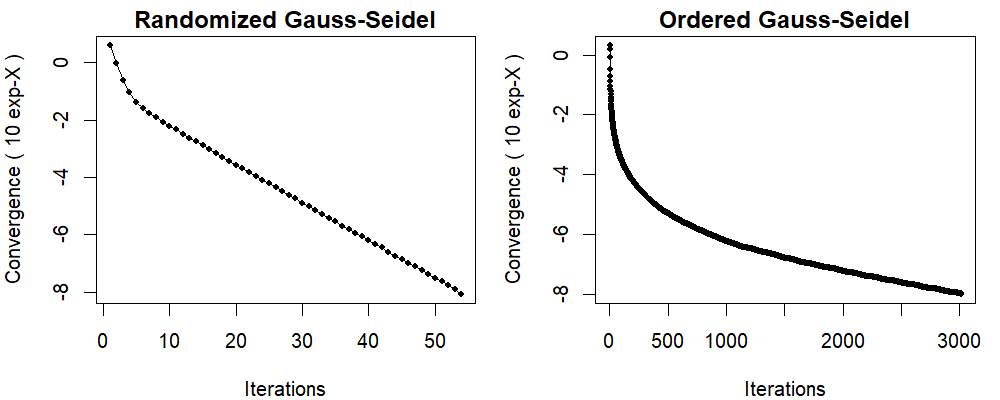
\includegraphics[width=12cm]{Figure1_rgs.png}
  \caption{\small{Convergence of the Gauss-Seidel solver with (left) and without (right) randomizing the order in which marker effects are updated for one replicate of the simulation of scenario 2.}}
  \label{convergence}
\end{figure}

Table \ref{RUNTIME2} depicts average runtime in minutes for PEGS, THGS, and UV-THGS with and without randomizing the marker order in the Gauss-Seidel solver as well as an increasing number of environments (scenario 4) and markers (scenario 5). PEGS and THGS had similar runtimes that were lower with randomization. Without randomization, the multivariate models that fitted 42,034 SNPs did not converge within 2,000 iterations.
Runtimes of PEGS and THGS increased exponentially with number of environments from 0.2 minutes for ten environments to 448 minutes for 400 environments using 4,311 SNPs. Runtime of UV-THGS, in contrast, increased linearly from 0.1 to 4.3 minutes under the same conditions. With randomization, runtime increased with increasing number of markers from 0.2 minutes for 4,311 SNPs to 0.8 minutes for 42,034 SNPs and ten environments, and from 80.5 to 123.2 minutes for 200 environments. Without randomization, runtime increased to 3,057.3 minutes for 42,034 SNPs and 200 environments.

\begin{table}[ht]
\centering
\renewcommand*{\arraystretch}{1.2}
\caption{Average runtime in minutes (s.e.) of the Gauss-Seidel solver with and without randomizing the order of markers for updating marker effects, with increasing number of SNPs and environments (envir.), and based on 10 replicates of scenarios 4 (4,311 SNPs) and 5 (42,034 SNPs).}\smallskip
\begin{tabular}{c c c c c c c}
 \hline
 Randomized & No. of SNPs & No. of envir. & PEGS & THGS & UV-THGS \\ 
 \hline
Yes &  4,311 &  10 & 0.2 (0) & 0.2 (0) & 0.1 (0) & \\
Yes &  4,311 &  50 & 3.5 (0.4) & 3.5 (0.4) & 0.6 (0) & \\
Yes &  4,311 & 100 & 14.4 (2) & 14.4 (1.8) & 1.1 (0) & \\
Yes &  4,311 & 200 & 80.5 (10.1) & 79.2 (11) & 2.3 (0.1) & \\
Yes &  4,311 & 400 & 459.3 (55.1) & 448 (58) & 4.3 (0.1) & \\
No &  4,311 &  10 & 5.5 (1) & 5.4 (0.9) & 1.9 (0.2) & \\
No &  4,311 &  50 & 44.9 (7) & 44.6 (6.9) & 9.3 (1.1) & \\
No &  4,311 & 100 & 120.9 (10.1) & 123.7 (9.9) & 20 (1.8) & \\
No &  4,311 & 200 & 361.1 (48.9) & 364.6 (44.4) & 39.3 (2.8) & \\
No &  4,311 & 400 & 1,261.8 (115.8) & 1,261.7 (107.9) & 74.1 (8.3) & \\
Yes & 42,034 &  10 & 0.8 (0.1) & 0.8 (0) & 1.2 (0.1) & \\
Yes & 42,034 &  50 & 9.9 (0.4) & 12.5 (1.3) & 5.7 (0.4) & \\
Yes & 42,034 & 100 & 36.4 (1.4) & 29.2 (2.7) & 11.3 (0.6) & \\
Yes & 42,034 & 200 & 123.2 (17.1) & 119.7 (10.1) & 22.5 (2) & \\
Yes & 42,034 & 400 & 730 (64.4) & 802.2 (118.2) & 46.4 (4.1) & \\
No & 42,034 &  10 & 64$^*$ (14.7) & 64.2$^*$ (16) & 14.5 (5.1) & \\
No & 42,034 &  50 & 540.2$^*$ (38.3) & 536$^*$ (26.8) & 106.5 (63.2) & \\
No & 42,034 & 100 & 1,109.6$^*$ (71.5) & 1,148.1$^*$ (109.3) & 181.4 (40.6) & \\
No & 42,034 & 200 & 3,057.3$^*$ (292.7) & 3,001.2$^*$ (259) & 310.3 (114.8) & \\
\hline
\multicolumn{4}{l}{\small{$^*$ Did not converge within 2,000 iterations.}} \\
\end{tabular}
\label{RUNTIME2}
\end{table}

\subsection{Accuracy and bias of GEBVs}

Accuracy of GEBVs increased with increasing heritability and genetic correlation, as expected (Figure \ref{Accuracy}). It was 0.03-0.09 higher for multivariate approaches than univariate THGS when heritability was low and genetic correlation medium to high (Figure \ref{Accuracy}, a and b, lower left panels). For most genetic parameters in scenario 1, REML provided 0.01 higher accuracy than PEGS and THGS. For low heritability and low genetic correlations, however, REML had 0.02 higher accuracy and UV-THGS was as accurate as PEGS and THGS (Figure \ref{Accuracy}a, upper left panel). The latter was also true for scenario 2. Upon further simulations of scenario 1 for low heritability and low genetic correlations, accuracies of PEGS and THGS became larger than UV-GS and approached those of REML with increasing number of environments (Section 2 of the supplement).
Compared to TVGS, even REML tended to have lower accuracies for low heritability and low genetic correlation (Figure \ref{Accuracy}a, upper left panel). The differences between TVGS and both PEGS and THGS were similar in scenarios 1 and 2 (Figure \ref{Accuracy}, a vs. b). PEGS and THGS were not significantly different in scenarios 1 and 2.
\\\\
Regression coefficients of TBV on GEBV are shown in Figure \ref{Slope}. For scenario 1 and low heritability, it was 1 for PEGS and THGS, close to 1 for REML, and significantly above 1 for UV-THGS. This bias for UV-THGS decreased with increasing heritability. For medium to high heritabilities, however, PEGS and THGS slightly underestimated (values $>$ 1) the TBVs, whereas REML was usually unbiased with value 1 (Figure \ref{Slope}a). The bias for PEGS and THGS decreased with increasing genetic correlation. In scenario 2 (Figure \ref{Slope}b), PEGS and THGS slightly overestimated TBVs (values $<$1) for low heritability, but slightly underestimated TBVs (values $>$1) for medium to high heritabilities. 

\begin{figure}[ht]
  %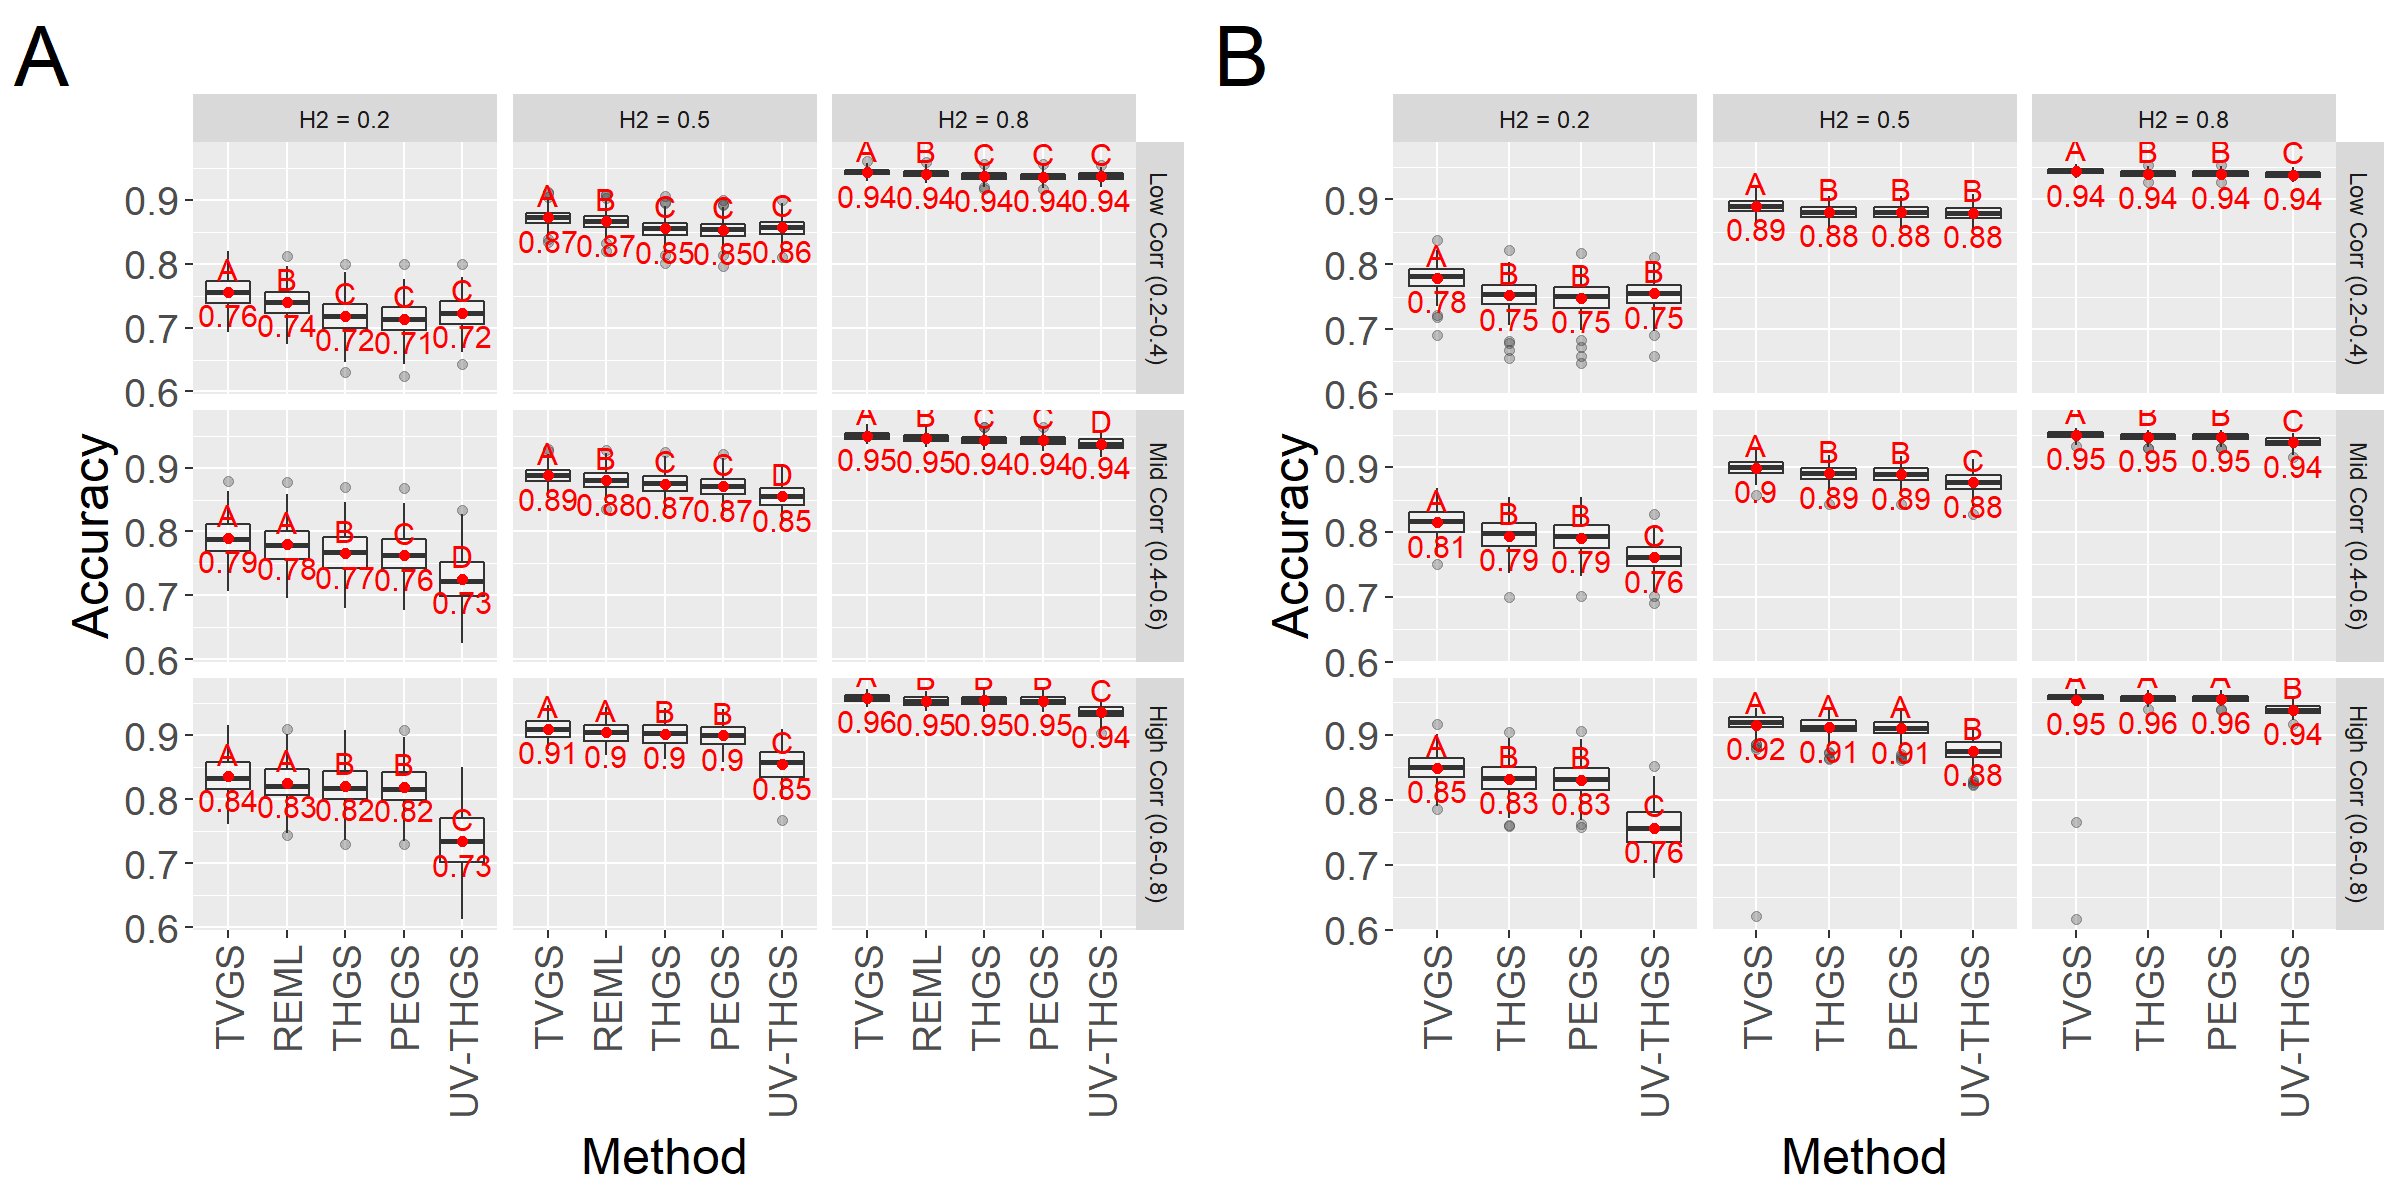
\includegraphics[width=12cm]{Figure2_acc.png}
  \caption{\small{Accuracy of GEBVs for scenario 1 (a, wheat dataset) and scenario 2 (b, soybean dataset) for different true heritabilities (columns) and genetic correlations (rows), based on 100 replicates of the simulation. Letters indicate Tukey's test of multiple comparisons ($\alpha=0.05$).}}
  \label{Accuracy}
\end{figure}

\begin{figure}[ht]
  %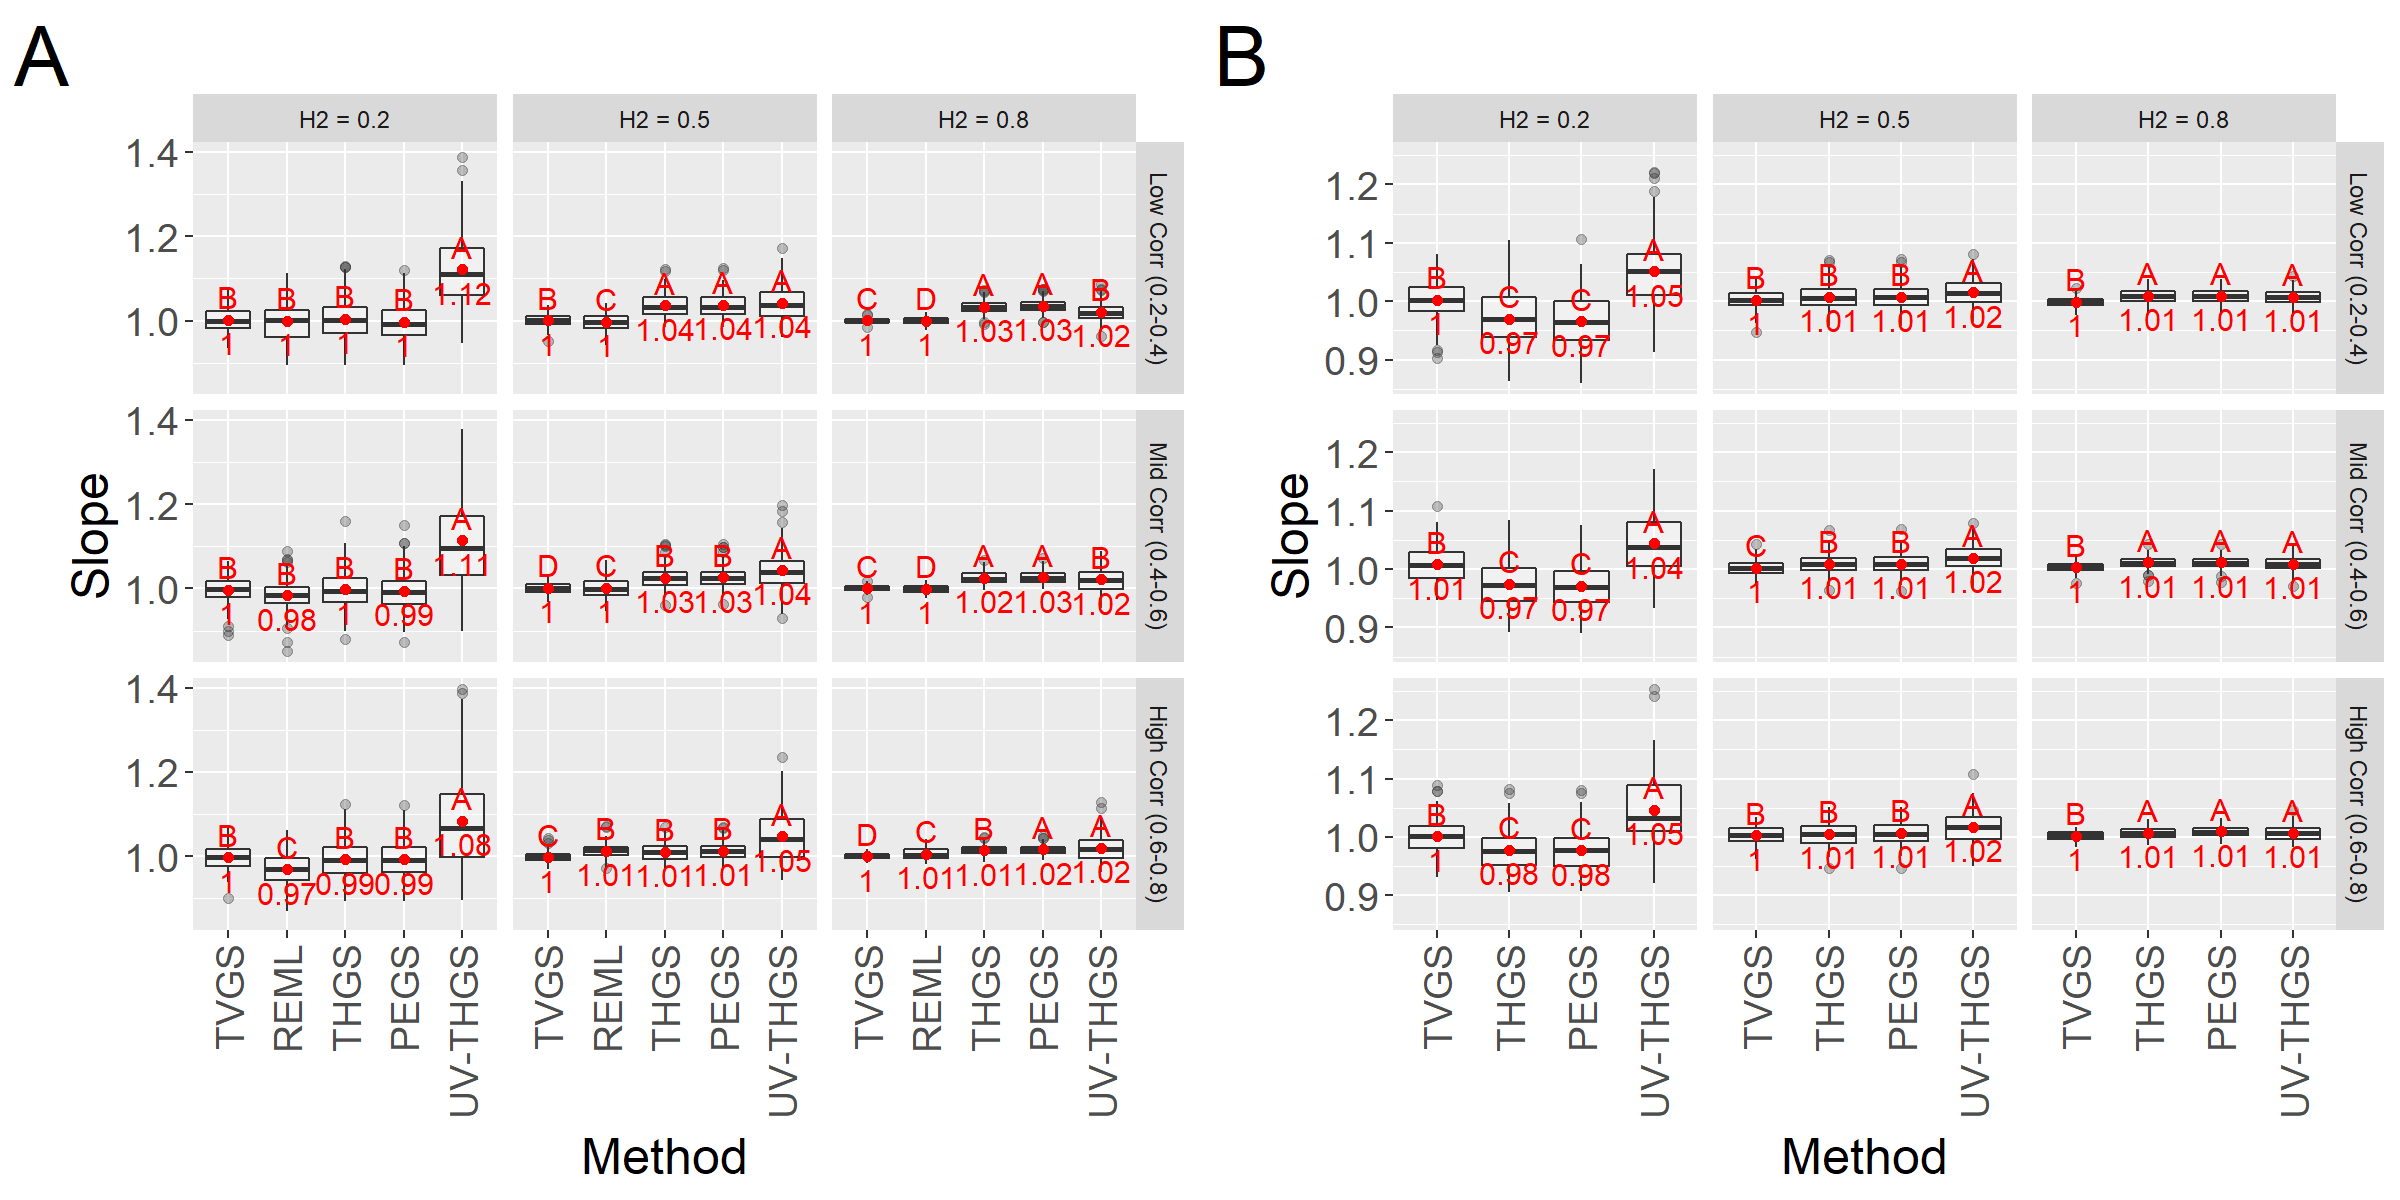
\includegraphics[width=12cm]{Figure3_slope.png}
  \caption{\small{Regression of true breeding values on GEBVs (slope) for scenario 1 (a, wheat dataset) and scenario 2 (b, soybean dataset) for different true heritabilities (columns) and genetic correlations (rows), based on 100 replicates of the simulation. Letters indicate Tukey's test of multiple comparisons ($\alpha=0.05$).}}
  \label{Slope}
\end{figure}

\subsection{Bias and standard error of estimated parameters}

Figure \ref{FigBiasH2} shows bias of estimated heritabilities for scenarios 1 and 2 and different genetic parameters. In both scenarios, heritabilities tended to be downward biased. The bias of PEGS and THGS was smallest or even zero for low heritability and medium to high genetic correlations (Figure \ref{FigBiasH2}, bottom left panels). Their biases decreased with increasing genetic correlations. The bias of UV-THGS tended to be lower than PEGS and THGS. REML provided the least biased heritability estimates in scenario 1. 

\begin{figure}%[!ht]
  %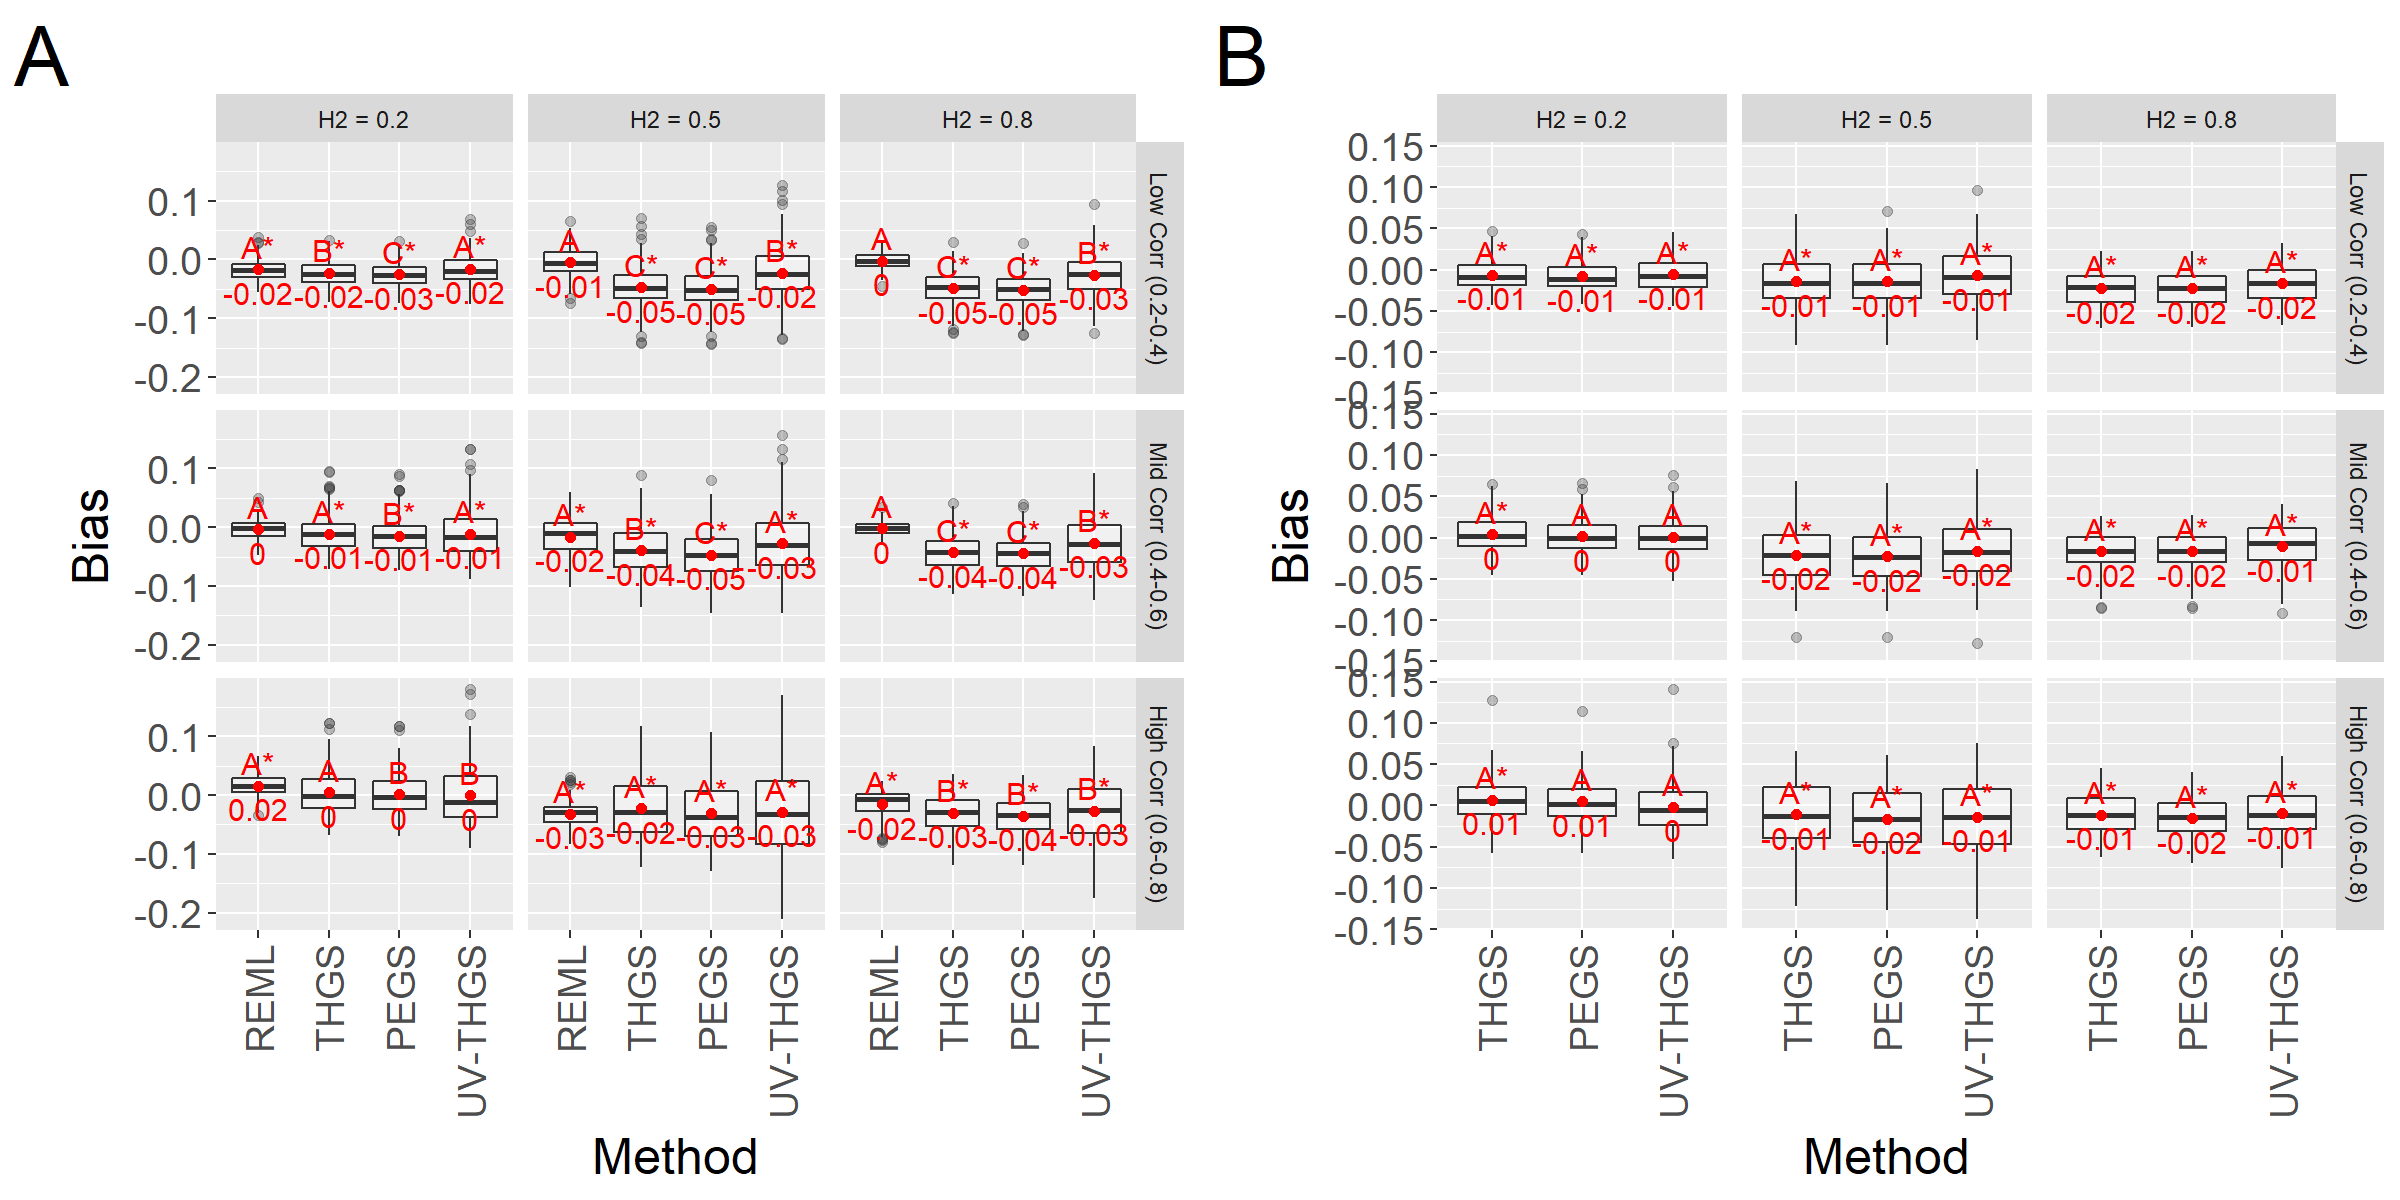
\includegraphics[width=12cm]{Figure4_h2bias.png}
  \caption{\small{Bias of estimated heritability for scenario 1 (a, wheat dataset) and scenario 2 (b, soybean dataset) for different true heritabilities (columns) and true genetic correlations (rows), based on 100 replicates of the simulation. Letters indicate Tukey's test  of multiple comparisons ($\alpha=0.05$). Asterisk indicates that the mean is significantly different from zero ($\alpha=0.05$).}}
  \label{FigBiasH2}
\end{figure}

Figure \ref{FigPrecH2} shows standard errors of estimated heritabilities for scenarios 1 and 2 and different genetic parameters. Standard errors were higher for scenario 1 than 2, higher for medium heritability than low and high heritabilities, highest for low genetic correlations, and decreased with increasing genetic correlation. They were between 60-100\% higher for PEGS and THGS than for REML.

\begin{figure}%[!ht]
  %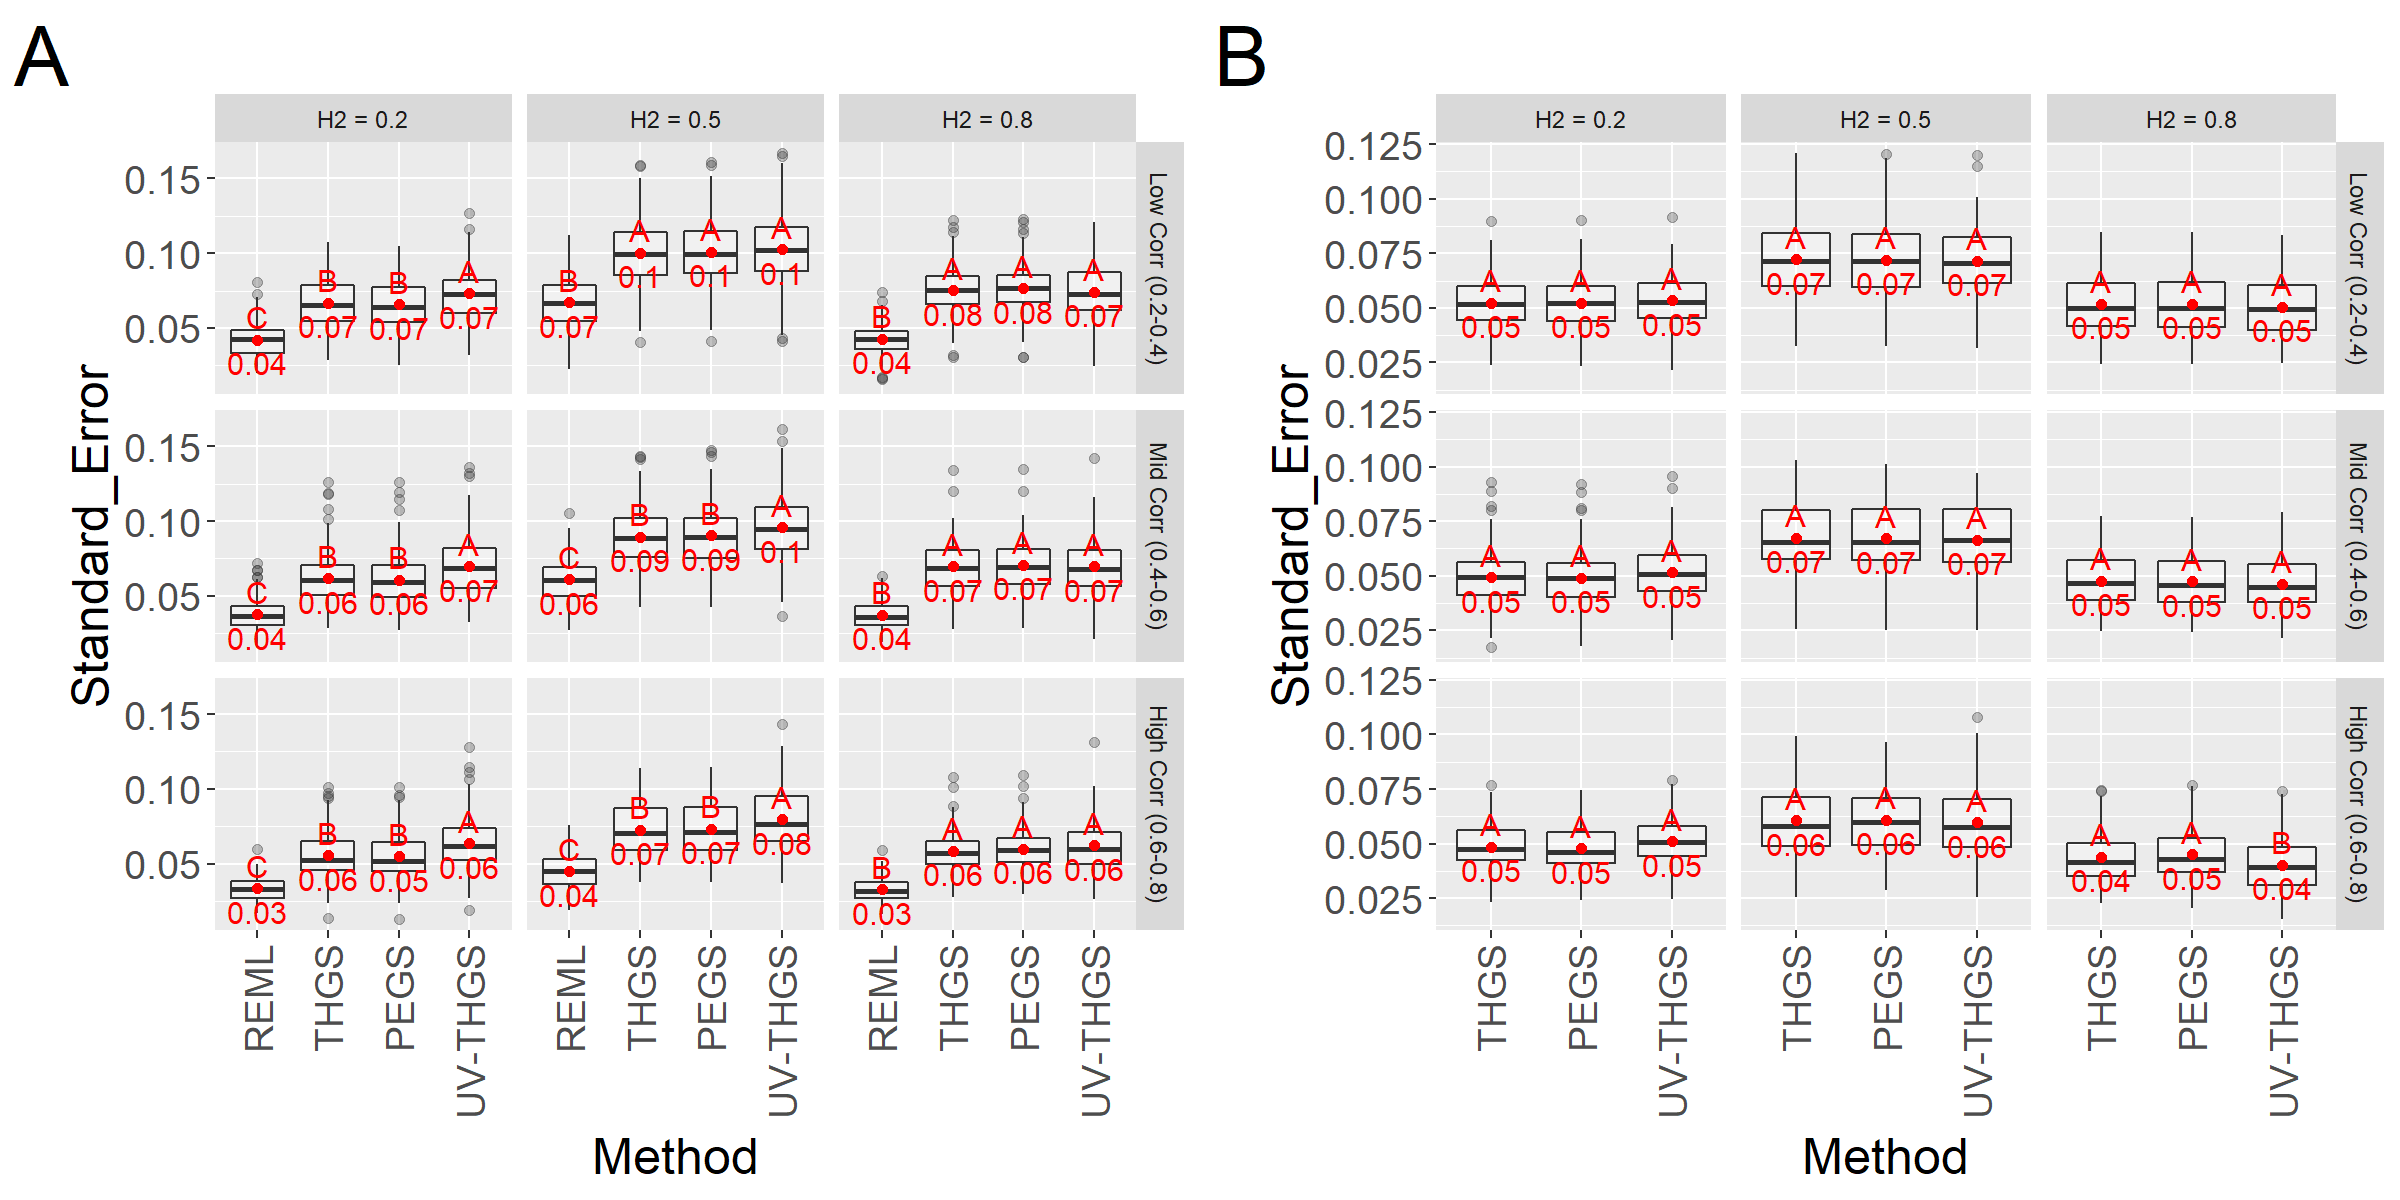
\includegraphics[width=12cm]{Figure5_h2se.png}
  \caption{\small{Standard error of estimated heritability for scenario 1 (a, wheat dataset) and scenario 2 (b, soybean dataset) for different true heritabilities (columns) and true genetic correlations (rows), based on 100 replicates of the simulation. Letters indicate Tukey's test of multiple comparisons ($\alpha=0.05$).}}
  \label{FigPrecH2}
\end{figure}

Figures \ref{GCBIAS} and \ref{GCSE} show bias and standard error of estimated genetic correlations for scenarios 1 and 2.  Bias tended to be low for PEGS and THGS in scenario 2, except for low heritability and high genetic correlations (Figure \ref{GCBIAS}b, lower left panel). In scenario 1 and for high genetic correlations (Figure \ref{GCBIAS}a, lower left panel), REML had large biases with absolute values of up to 0.08, compared to 0.01 for THGS. Otherwise, REML and the proposed methods had similar biases, and they were not significantly different for PEGS and THGS. As standard software for REML did not return results for the full model and the  unbalanced designs in scenario 2, bivariate models were ran and estimated genetic correlations are given in section 3 of the supplement.

\begin{figure}%[!ht]
  %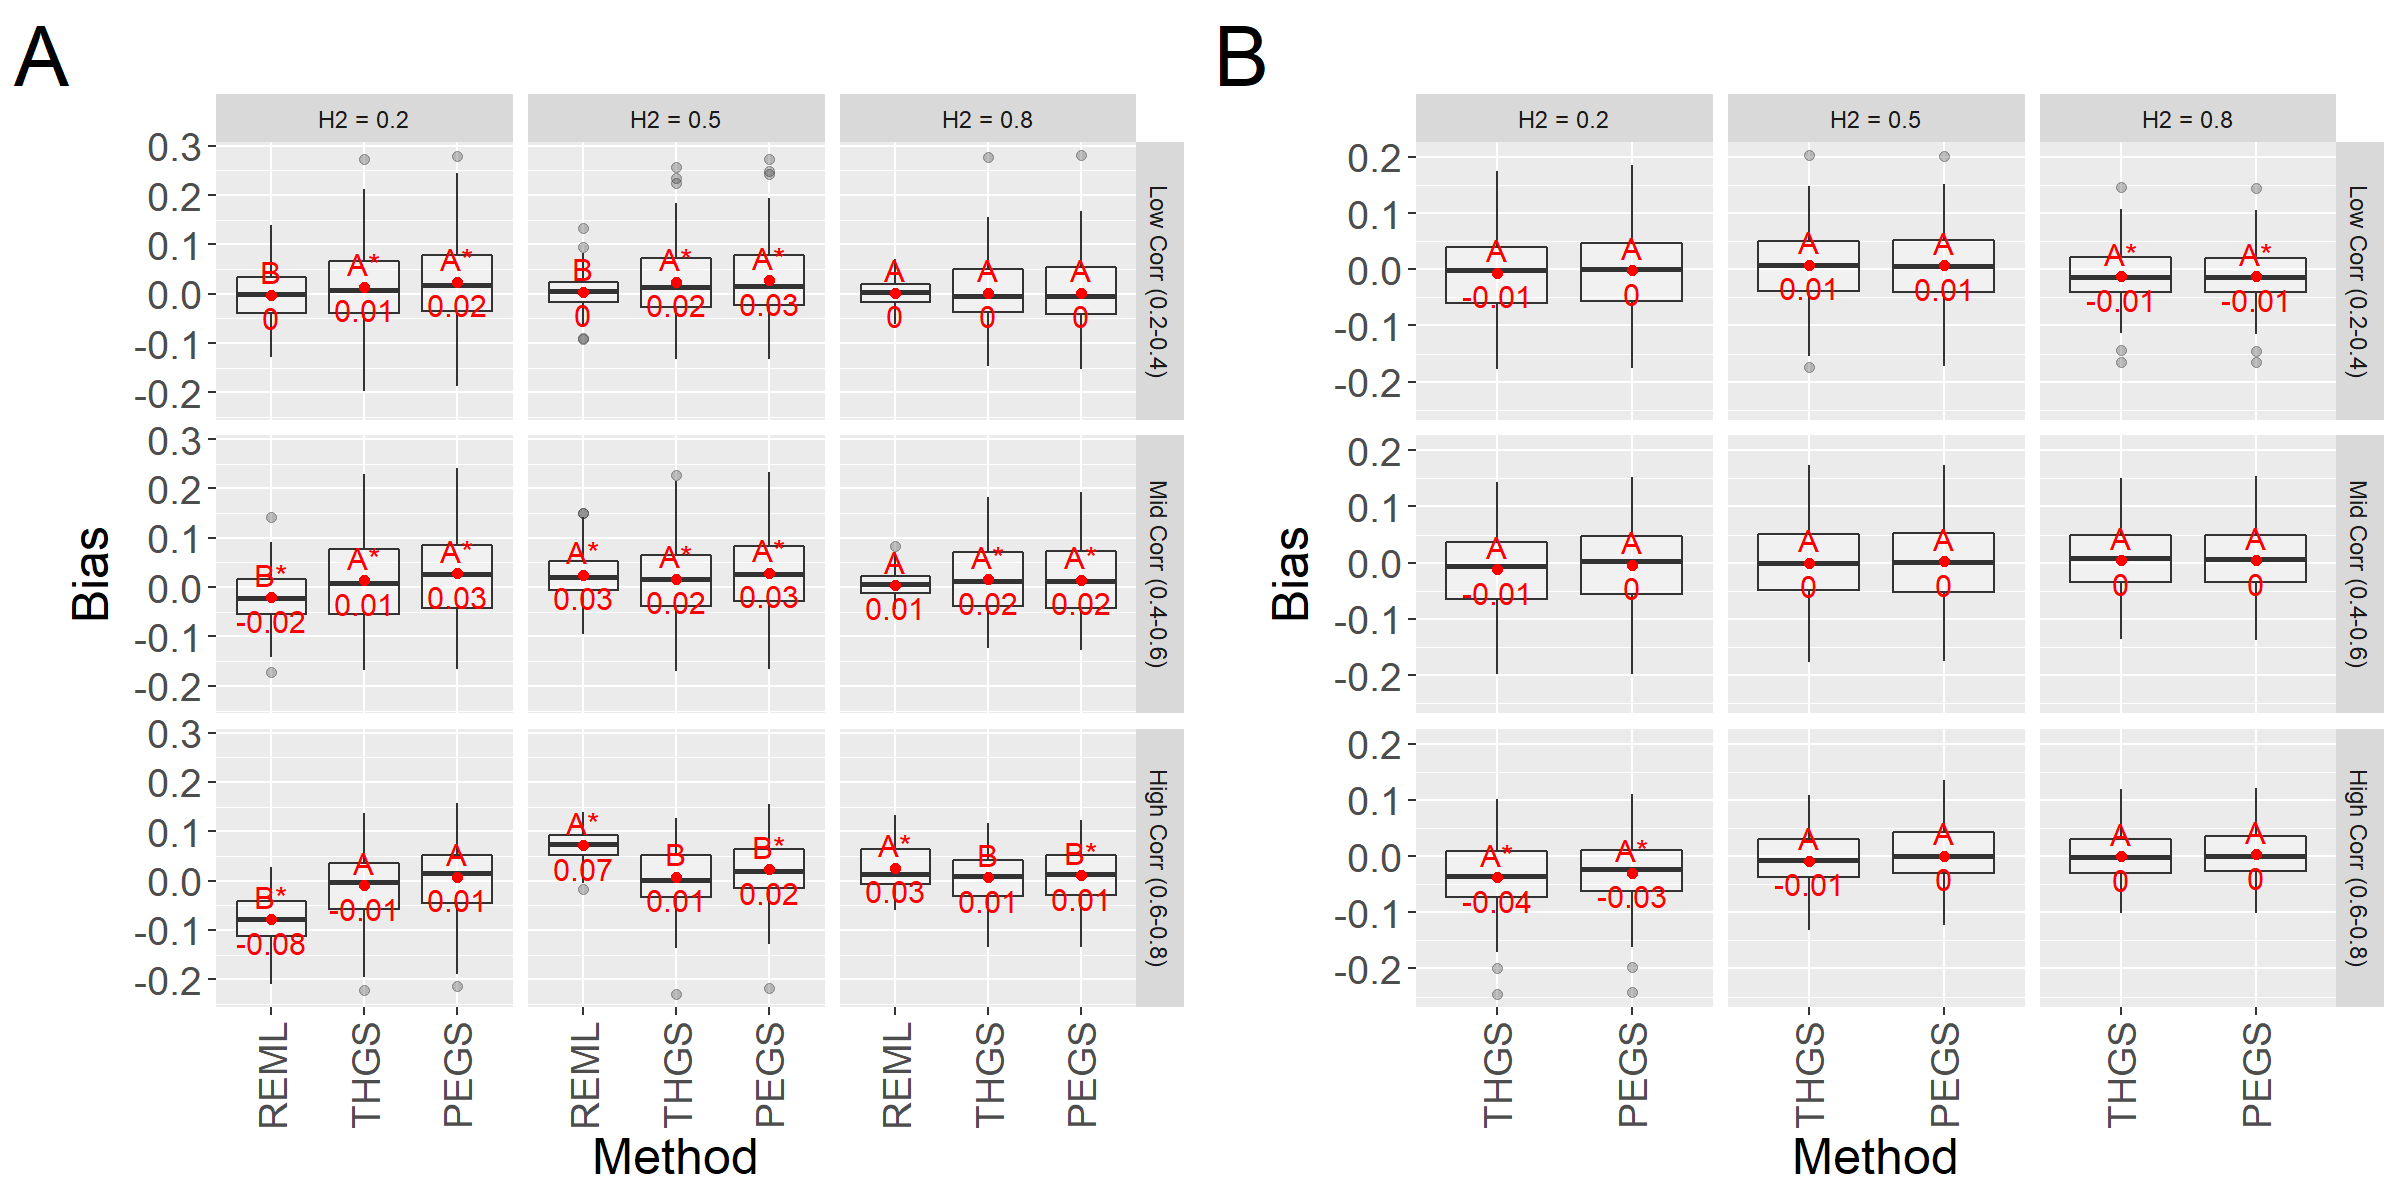
\includegraphics[width=12cm]{Figure6_gcbias.png}
  \caption{\small{Bias of estimated genetic correlations for scenario 1 (a, wheat dataset) and scenario 2 (b, soybean dataset) for different true heritabilities (columns) and true genetic correlations (rows), and based on 100 replicates of the simulation. Letters indicate Tukey's test of multiple comparison ($\alpha=0.05$). Asterisk indicates that the mean is significantly different from zero ($\alpha=0.05$).}}
  \label{GCBIAS}
\end{figure}

Standard errors of estimated genetic correlations decreased with increasing heritability and genetic correlations (Figure \ref{GCSE}). Values of PEGS and THGS were always similar, but higher than for REML for low to medium genetic genetic correlations. For high genetic correlations, standard errors were similar for all methods. Standard errors were lower for scenario 2 than 1.

\begin{figure}%[!ht]
  %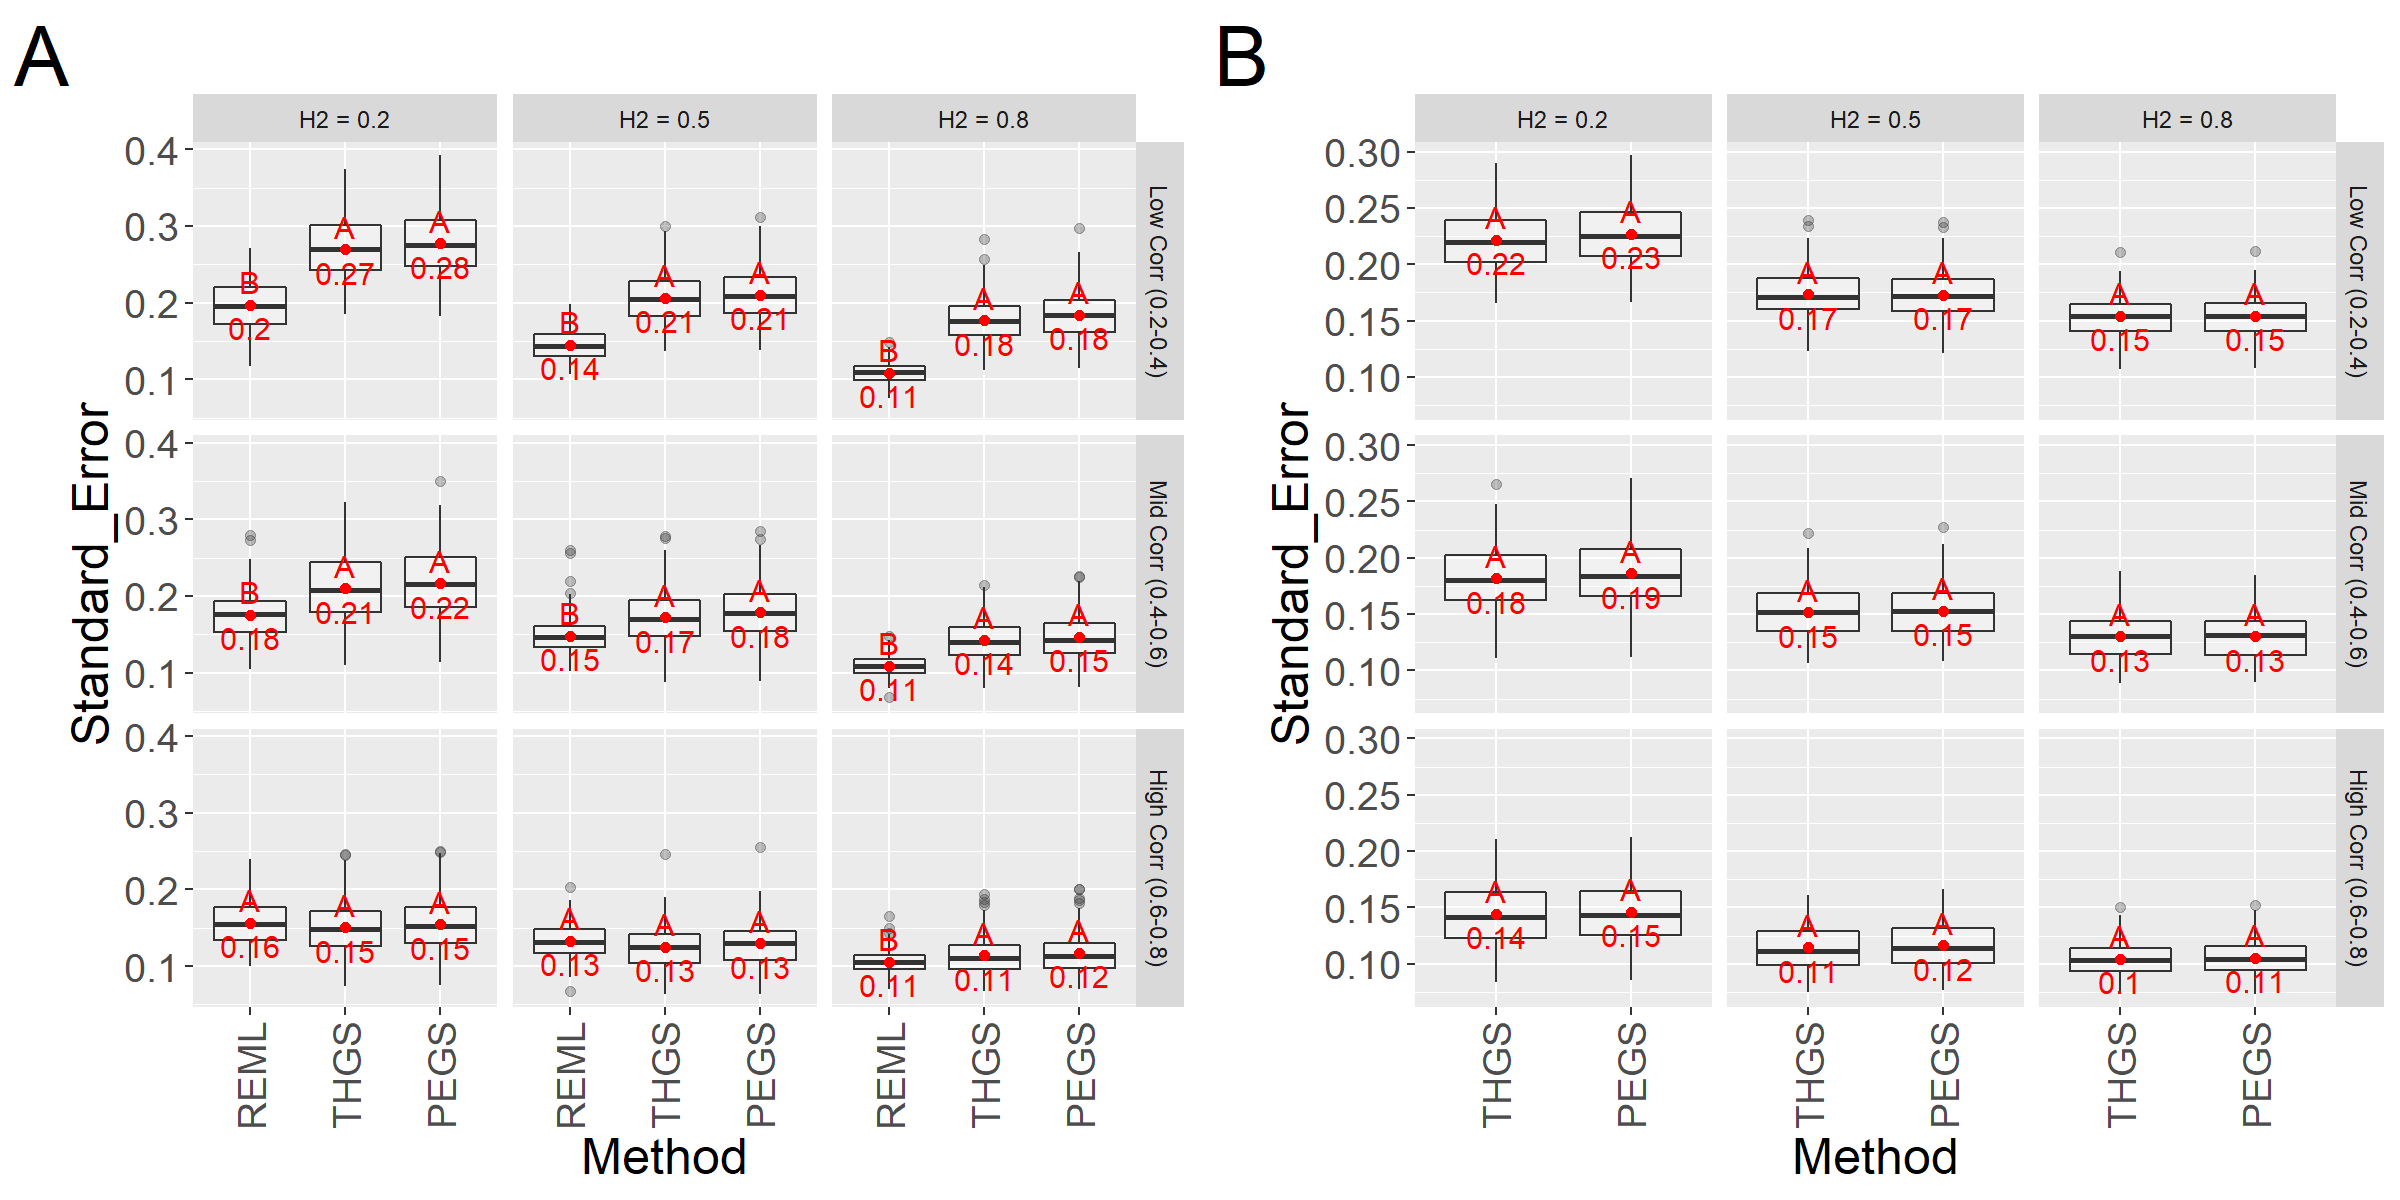
\includegraphics[width=12cm]{Figure7_gcse.png}
  \caption{\small{Standard error of estimated genetic correlations for scenario 1 (a, wheat dataset) and scenario 2 (b, soybean dataset) for different true heritabilities (columns) and true genetic correlations (rows), based on 100 replicates of the simulation. Letters indicate Tukey's test of multiple comparisons ($\alpha=0.05$). Asterisk indicates that the mean is significantly different from zero ($\alpha=0.05$).}}
  \label{GCSE}
\end{figure}

As the number of observations per environment increased in scenario 3, standard errors of estimated genetic parameters decreased, bias of estimated genetic correlations decreased, but bias of heritabilities did not approach zero even with 3,000 observations per environment (Table \ref{VaryN}). Section 4 of the supplement demonstrates the outcome when all 5,142 individuals were observed in all environments: heritabilities estimated with THGS were unbiased, and genetic correlations estimated with PEGS or THGS were unbiased.

\begin{table}[ht]
\centering
\renewcommand*{\arraystretch}{1.2}
\caption{Accuracy of GEBVs, regression of TBV on GEBV (Slope), and bias and standard error (SE) of estimated heritabilities ($\hat{h}^2$) and genetic correlations (GC) with increasing number of observations per environment (Obs/Env) in scenario 3, based on 100 replicates of the simulation. Standard errors of statistics are in parenthesis.}\smallskip
\begin{tabular}{l c c c c c c c}
 \hline
Method & Obs/Env & Accuracy & Slope & Bias of $\hat{h}^2$ & SE of $\hat{h}^2$ & Bias of GC& SE of GC \\
 \hline
PEGS & 250 & 0.82 (0.03) & 0.98 (0.03) & -0.01 (0.03) & 0.07 (0.01) & -0.01 (0.06) & 0.17 (0.02) \\
PEGS & 3000 & 0.96 (0.03) & 1.00 (0.03) & -0.01 (0.03) & 0.04 (0.01) & 0.00 (0.06) & 0.13 (0.02) \\
THGS & 250 & 0.82 (0.03) & 0.98 (0.04) & 0.00 (0.03) & 0.07 (0.01) & -0.02 (0.06) & 0.17 (0.02) \\
THGS & 3000 & 0.96 (0.03) & 1.00 (0.03) & -0.01 (0.03) & 0.04 (0.01) & 0.00 (0.06) & 0.13 (0.02) \\
UV-THGS & 250 & 0.79 (0.03) & 1.04 (0.03) & -0.01 (0.03) & 0.07 (0.01) & - & - \\
UV-THGS & 3000 & 0.95 (0.03) & 1.00 (0.04) & -0.01 (0.03) & 0.04 (0.01) & - & - \\
 \hline
\end{tabular}
\label{VaryN}
\end{table}

\subsection{Orthogonalization}

Table \ref{ExTH} presents bias and accuracy of GEBVs as well as bias and standard error of estimated genetic parameters with and without using eigenvalue decomposition (EVD). THGS-EVD provided unbiased GEBVs (Slope = 1) and its accuracy was 0.01 higher than THGS and thus equal to the accuracy of REML. Estimated genetic correlations of THGS-EVD were unbiased and had lower standard errors than THGS. The accuracy of GEBVs from UV-THGS-EVD did not increase compared to UV-THGS, suggesting that the increase of accuracy for THGS-EVD resulted from a higher precision in estimating genetic correlations. PEGS and PEGS-EVD were not different.

\begin{table}[ht]
\centering
\renewcommand*{\arraystretch}{1.2}
\caption{Accuracy of GEBVs, regression of TBV on GEBV (Slope) as well as bias and standard error (SE) of estimated heritabilities ($\hat{h}^2$) and genetic correlations (GC) with eigenvalue decomposition (EVD) and without, based on 100 replicates of the simulation of scenario 1.}\smallskip
\begin{tabular}{l c c c c c c c }
\hline
Method & Accuracy & Slope  & Bias of $\hat{h}^2$ & SE of $\hat{h}^2$ & Bias of GC & SE of GC   \\
\hline
REML-EVD & 0.87 (0.02) & 1.00 (0.03) & -0.01 (0.02) & 0.04 (0.01) & 0.00 (0.04) & 0.14 (0.03) \\
PEGS & 0.86 (0.02) & 1.02 (0.03) & -0.03 (0.04) & 0.07 (0.02) & 0.02 (0.08) & 0.18 (0.04) \\
PEGS-EVD & 0.86 (0.02) & 1.02 (0.03) & -0.04 (0.04) & 0.07 (0.02) & 0.02 (0.08) & 0.18 (0.04) \\
THGS & 0.86 (0.02) & 1.02 (0.03) & -0.03 (0.04) & 0.07 (0.02) & 0.01 (0.08) & 0.17 (0.04) \\
THGS-EVD & 0.87 (0.02) & 1.00 (0.03) & -0.02 (0.03) & 0.05 (0.01) & 0.00 (0.04) & 0.13 (0.02) \\
UV-THGS & 0.84 (0.04) & 1.06 (0.09) & -0.02 (0.05) & 0.08 (0.02) & - & - \\
UV-THGS-EVD & 0.84 (0.03) & 1.03 (0.04) & -0.03 (0.03) & 0.05 (0.01) & - & - \\
\hline
\end{tabular}
\label{ExTH}
\end{table}


\section{Discussion}

Our main goal was to find an algorithm for multivariate genomic prediction, which is efficient in runtime and memory, applicable to unbalanced experimental designs, and exploits genetic correlations between environments to increase accuracy of GEBVs compared to univariate analyses. We proposed two algorithms, PEGS and THGS, that use Randomized Gauss-Seidel to solve marker effects and simultaneously estimate variance components with methods developed by \cite{Schaeffer} and \cite{VanRaden}, respectively. Simulations were conducted to evaluate bias and accuracy of GEBVs within environment and compare them to those obtained by REML and a univariate approach. Bias and standard error of estimated heritabilities and genetic correlations were also evaluated to interpret the differences in bias and accuracy of GEBVs between methods (Table \ref{METHODS}).

PEGS and THGS are fast and memory-efficient algorithms for both balanced and unbalanced experimental designs, and had much lower runtime than REML using standard software implementations (Tables \ref{RUNTIME1} and \ref{RUNTIME2}). Moreover, they are scalable with number of environments and markers. The reasons for the speed-up are that equations are solved by Randomized Gauss-Seidel and that expectations of quadratic forms, shown in the denominator of equations (\ref{eqn:SigmaBk}) and (\ref{eqn:SigmaBij}), are inexpensive to compute. These expectations do not require elements of the inverse of the left-hand side of the mixed-model equations as shown in \cite{Schaeffer}. Therefore, the system of equations essentially reduces to a $K\times K$ problem (equation \ref{eqn:GS_B}) with complexity $O(K^3)$. When hundreds to thousands of response variables were to be fitted at once, it is possible to linearize operations through a full-conditional multivariate Gauss-Seidel algorithm presented in Appendix \ref{UVMVsol}.

The number of iterations to convergence (Figure \ref{convergence}) and thereby runtime of PEGS and THGS decreased greatly by randomizing the marker order for updating marker effects (Table \ref{RUNTIME2}).  This may be due to reducing dependencies among markers that stem from high linkage disequilibrium between adjacent markers on the same chromosome. With an increasing number of environments and markers, PEGS and THGS have reasonably low runtimes (Table \ref{RUNTIME2}, with randomization), which allows breeders to make decisions on time, and rerun genetic evaluations as data become available during harvest season.

For balanced designs, the number of iterations to convergence can be further reduced by modeling the eigenvectors of genotype scores, which completely removes dependencies among model effects. In addition, THGS becomes an exact method that yields unbiased estimates of genetic correlations and GEBVs (section 2.4), and reduces the bias of estimated heritabilities as can be demonstrated for scenario 1 (Table \ref{ExTH}). Matrix decomposition is also useful to analyze high-dimensional datasets with many factors ($P>>N$ problem), and to fit one or multiple kernels of different types within a multivariate ridge regression model. For example, for modeling dominance, epistasis \cite{Xu2013}, Gaussian or Arc-cosine relationships \cite{Xavier2021,Kernel2021}. The computing costs for matrix decomposition to obtain those eigenvectors, however, may outweigh the benefits for THGS with an increasing number of individuals and markers in the analysis.

The trade-off for higher speed is a slightly lower accuracy of GEBVs of 0.01 compared to REML under realistic conditions when heritability was low and genetic correlations between environments were medium to high (Figure \ref{Accuracy}a). PEGS and THGS exploited genetic correlations between environments under these conditions and had higher accuracy of GEBVs than the univariate approach (Figure \ref{Accuracy}a and b). Only in the worst case, when all heritabilities and all genetic correlations between environments were low, the benefit of multivariate genomic prediction for achieving a higher accuracy than the univariate approach vanished with PEGS and THGS (Figure \ref{Accuracy}a and b). The reason is a lower precision in estimating genetic correlations as their standard errors were notably higher for PEGS and THGS than for REML (Figure \ref{GCSE}). Moreover, PEGS and THGS slightly underestimated heritabilities and slightly overestimated genetic correlations. The bias of GEBVs, however, was close to zero and approached zero with increasing number of individuals per environment (Figure \ref{Slope}, Table \ref{VaryN}, Appendix \label{AppTab}).

Residuals were treated as uncorrelated between environments for three reasons. First, the phenotypes come from different plants that are assumed to have uncorrelated environmental effects in their residuals. Second, epistatic effects, which are not captured by the marker effects in the model of equation (\ref{eqn:StatModel}), are assumed to have small covariances between environments. Third, the PEGS and THGS algorithms are faster because the absorption matrix $\mat{M}$, which is used in equations \ref{BetaTilde}-\ref{eqn:SigmaEk}, is block-diagonal with one block per environment, $\mat{M}_k$. In addition, fewer computations are required to update estimated marker effects when the residual covariance matrix is diagonal (see equation \ref{eqn:GS_B}). If phenotypes come from multiple quantitative traits, residual covariances may need to be modeled to avoid further bias in estimated genetic parameters and GEBVs, which may increase runtime \cite{Schaeffer} and offset the computational advantage compared to REML. However, these covariances could be modeled with an additional random term constructed by the cross-product of sparse 0/1-incidence matrices for genotypes from different environments. Otherwise, the effect of neglecting residual covariances on bias of genetic parameters and GEBVs could be evaluated on a case-by-case basis.

%This is a standard assumption in plant breeding \cite{TwoStage1,TwoStage2} 

Estimated variances and covariances from the methods PE and TH are unbiased when the mixed-model equations are weighted by the true variances and covariances as shown in section 1 of the supplement and Appendix \ref{EVTH}. In practice, however, an iterative procedure starts with best guesses for genetic parameters, and thus estimates are not expected to be unbiased, which is identical to REML or iterative MIVQUE \cite{Searle1992}. As discussed in \cite{VanRaden}, estimates may be further biased when populations are under selection. This was not considered here because plant-breeding datasets used for genomic prediction may not contain selection if they are properly augmented by unselected genotypes or designed to maximize prediction accuracy \cite{HabierOpt2013,Rincent2017}. Furthermore, data may come from a single selection stage and thereby do not contain selection information. Yet, Ouweltjes et al. \cite{Ouweltjes1988} and VanRaden and Jung \cite{VanRaden} found that PE can be more suitable than TH for selected data, but both methods are more biased than REML. These studies were performed using pedigree information and the bias was attributed to neglecting off-diagonals of the relationship matrix. To better understand this, the original quadratic form, $\hat{\vecx{\beta}}'_k\hat{\vecx{\beta}}_k$, can be compared to $\tilde{\vecx{\beta}}'_k\hat{\vecx{\beta}}_k$ from equation (\ref{eqn:SigmaBk}). For ease of explanation, only the univariate case and the method PE with $\tilde{\vecx{\beta}}_k = \mat{Z}'_k\mat{M}_{k} \vecx{y}_k$ is considered here. Using BLUP formulas \cite{Searle1992BLUP}, the quadratic forms can be written as
\begin{align}\label{QFORMS1}
    \hat{\vecx{\beta}}'_k\hat{\vecx{\beta}}_k &= (\vecx{y}_k-\mat{X}\hat{\vecx{b}}_{\textrm{GLS}_k})'\mat{V}^{-1}_k\mat{Z}_k\sigma^2_{\beta_k}\sigma^2_{\beta_k}\mat{Z}'_k\mat{V}^{-1}_k(\vecx{y}_k-\mat{X}\hat{\vecx{b}}_{\textrm{GLS}_k}),
\end{align}
and
\begin{align}\nonumber
    \tilde{\vecx{\beta}}'_k\hat{\vecx{\beta}}_k &= \vecx{y}'_k\mat{M}_k\mat{Z}_k
    \hat{\vecx{\beta}}_k\\\label{QFORMS2}
    &= (\vecx{y}_k-\mat{X}\hat{\vecx{b}}_{\textrm{LS}_k})'\mat{Z}_k\sigma^2_{\beta_k}\mat{Z}'_k\mat{V}^{-1}_k(\vecx{y}_k-\mat{X}\hat{\vecx{b}}_{\textrm{GLS}_k}),
\end{align}
where $\mat{V}^{-1}_k$ is the inverse of the variance-covariance matrix of $\vecx{y}_k$, $\mat{V}_k = \mat{Z}_k\mat{Z}'_k\sigma^2_{\beta_k}+\mat{I}\sigma^2_{e_k}$, and $\hat{\vecx{b}}_{\textrm{GLS}_k}$ and $\hat{\vecx{b}}_{\textrm{LS}_k}$ are the Generalized Least Squares and Least Squares estimators of $\vecx{b}$, respectively. Thus in $\tilde{\vecx{\beta}}_k$, the matrix $\mat{V}^{-1}_k$, which contains genomic relationships between individuals, i.e., $\mat{Z}_k\mat{Z}'_k$, is not used to weigh $\vecx{y}_k$, neither for estimating fixed effects ($\hat{\vecx{b}}_{\textrm{LS}_k}$) nor random effects. However, THGS in combination with a Principal components or an eigenvector regression does not have this issue and can be used for balanced datasets with selection.

PEGS and THGS should be evaluated against alternative methods that are commonly used in plant breeding for modeling phenotypes from multiple environments. These are compound symmetry and extended factor analytic (XFA) models \cite{MeyerXFA}. Compound symmetry models fit a term for the average genetic effect of an individual across environments and another term for the specific environmental effects for an individual. As each term is modeled with only one variance, this model assumes that the genetic correlations between all pairs of environments are identical. The difference between that single correlation and the true correlation between any one pair can be regarded as bias. The XFA model fits more parameters than the compound symmetry model to reduce this bias, but less parameters than an unstructured multivariate model that fits a correlation for each pair of environments. XFA models thereby balance bias and precision of estimated genetic correlations. Therefore, these two alternative models tend to bias estimated genetic correlations between environments and are expected to decrease accuracy of GEBVs compared to estimating genetic correlations between all pairs of environments.

The iterative algorithm of PEGS and THGS differs from that of REML and Bayesian Gibbs sampling. In each iteration of REML, the mixed-model equations are fully solved to obtain estimates of the model effects conditional on the current variance components of that iteration. The estimated model effects are then used to update the variance components and a new iteration begins unless the change in variance components is small. In PEGS and THGS, in contrast, the model effects are merely updated, not solved, before variance components are updated and a new iteration begins. In Bayesian Gibbs sampling, similar computations are conducted in each iteration as in PEGS and THGS. However, rather than converging directly to a solution within a small number of iterations, the Gibbs algorithm samples from the posterior for thousands of iterations, and therefore must have longer runtimes. 

\section{Conclusion}

%Needs more thought, just an attempt to bring in my thoughts

PEGS and THGS are fast, memory-efficient, and reliable algorithms for genomic prediction for both balanced and unbalanced experimental designs. They are scalable with increasing number of response variables and markers. Their runtime is much lower than for REML and Gibbs sampling. For balanced designs, THGS provides unbiased GEBVs and estimated genetic correlations if only an intercept is modeled, and eigenvalue decomposition is feasible. Without eigenvalue decomposition, the accuracy of GEBVs of PEGS and THGS is slightly lower than REML, but higher than univariate THGS under realistic genetic correlations among environments. Estimated genetic parameters have little bias, but the standard errors are larger than for REML. More studies are needed to evaluate them for unbalanced datasets with selection. 

\begin{backmatter}

\section*{Ethics approval and consent to participate}
Not applicable.

\section*{Consent for publication}
Not applicable.

\section*{Availability of data and materials}
Genotypic data of the wheat dataset are available in the R package BGLR using the command \mintinline{MySQL}{data(wheat,package='BGLR')}, and genotypic data of the SoyNAM dataset are available in the R package SoyNAM using the command \mintinline{MySQL}{data <- SoyNAM::ENV()}. An implementation of PEGS is provided in the R package bWGR (2.0), function \textbf{mrr}.

\section*{Competing interests}
The authors declare that they have no competing interests.

\section*{Funding}
The authors are salaried researchers. No particular funding was provided for this research. 

\section*{Author's contributions}
AX and DH developed the methods, implemented the algorithms, planned the validations, wrote the manuscript.

\section*{Acknowledgements}
Not applicable.

% if your bibliography is in bibtex format, use those commands:
\bibliographystyle{bmc-mathphys} % Style BST file (bmc-mathphys, vancouver, spbasic).
%\\ \bibliography{bmc_article}      % Bibliography file (usually '*.bib' )
% for author-year bibliography (bmc-mathphys or spbasic)
% a) write to bib file (bmc-mathphys only)
% @settings{label, options="nameyear"}
% b) uncomment next line
%\nocite{label}

\bibliography{bmc_article}

\newpage

\end{backmatter}

\appendix

\section{Efficient calculation of $\mat{Z}'_{k} \mat{M}_{k} \mat{Z}_{k}$ and  $\mat{M}_{k}\vecx{y}_k$\label{byPassM}}

Only the diagonal elements of  $\mat{Z}'_{k} \mat{M}_{k} \mat{Z}_{k}$ are needed as matrix $\mat{D}_k$ is diagonal (equation \ref{MatrixD}). They can be computed one at a time for environment $k$ and marker $j$ as
\begin{equation}\nonumber
\label{eqn:TrZMZ}
\vecx{z}'_{jk} \mat{M}_{jk} \vecx{z}_{k}  = \vecx{z}_{jk}'\vecx{z}_{jk} - \vecx{z}_{jk}'\mat{X}_{k}(\mat{X}'_{k} \mat{X}_{k})^{-1} \mat{X}'_{k} \vecx{z}_{jk}
\end{equation}
where $(\mat{X}'_{k} \mat{X}_{k})^{-1}$ is computed once before iterations start. Likewise, $\mat{M}_{k}\vecx{y}_k$ of equation \ref{eqn:SigmaEk} can be obtained once as 
\begin{equation}\nonumber
\label{eqn:My}
\mat{M}_{k}\vecx{y}_k = \vecx{y}_k - \mat{X}_{k}(\mat{X}'_{k} \mat{X}_{k})^{-1} \mat{X}'_{k} \vecx{y}_k = \vecx{y}_k - \mat{X}_{k} \vecx{\hat{b}}_{LS_k},
\end{equation}
where $\vecx{\hat{b}}_{LS_k}$ denotes the Least Squares estimate of $\vecx{b}$.


\section{Expected value of $\tilde{\vecx{\beta}}'_k\hat{\vecx{\beta}}_k$\label{EVTH}}

Let $\tilde{\vecx{\beta}}_k = \mat{D}^{-1}_k\mat{Z}'_k\mat{M}_k\vecx{y}_k$ and $\mat{M}_k = \mat{I}_k - \mat{X}_k(\mat{X}'_k\mat{X}_k)^{-1}\mat{X}_k$, as defined in section 2.3, and let $\hat{\vecx{\beta}}_k = \sigma^2_{\beta_k}\mat{Z}'_k\mat{P}_k\vecx{y}_k$ be the Best Linear Unbiased Predictor (BLUP) of $\vecx{\beta}$ \cite{Searle1992BLUP}, where $\mat{P}_k = \mat{V}^{-1}_k[\mat{I}_k-\mat{X}_k(\mat{X}'_k\mat{V}^{-1}_k\mat{X}_k)^{-1}\mat{X}_k\mat{V}^{-1}_k]$ and $E(\hat{\vecx{\beta}}) = \vecx{0}$. Then, the expected value of the bilinear form  $\tilde{\vecx{\beta}}'_k\hat{\vecx{\beta}}_k$ \cite{Searl71} is
\begin{align*}
    E(\tilde{\vecx{\beta}}'_k\hat{\vecx{\beta}}_k) &= tr(Cov(\tilde{\vecx{\beta}}_k, \hat{\vecx{\beta}}'_k)) + E(\tilde{\vecx{\beta}}_k)'E(\hat{\vecx{\beta}}_k)\\
    &= tr(\mat{D}^{-1}_k\mat{Z}'_k\mat{M}_k\mat{V}_k\mat{P}_k\mat{Z}_k\sigma^2_{\beta_k})\\
    &= tr(\mat{D}^{-1}_k\mat{Z}'_k\mat{M}_k\mat{Z}_k)\sigma^2_{\beta_k},
\end{align*}
because $\mat{M}_k\mat{V}_k\mat{P}_k = \mat{M}_k$. Hence, 
\begin{align*}
    \hat{\sigma}^2_{\beta_k} &= \frac{\tilde{\vecx{\beta}}'_k\hat{\vecx{\beta}}_k}{tr(\mat{D}^{-1}_k\mat{Z}'_k\mat{M}_k\mat{Z}_k)},
\end{align*}
and $E(\hat{\sigma}^2_{\beta_k}) = \sigma^2_{\beta_k}$. The extension to using $\hat{\vecx{\beta}}_k$ from a multivariate BLUP is presented in section 1 of the supplement.

\section{Equivalence of $\hat{\vecx{\beta}}$ and $\tilde{\vecx{\beta}}$ using EVD} \label{ExactTH}

Let the eigenvalue decomposition of $\mat{Z}'_k\mat{Z}_k$ be
$\mat{U}_k\mat{\Lambda}_k\mat{U}'_k$, where $\mat{U}_k$ is an orthonormal matrix of eigenvectors with the property $\mat{U}'_k\mat{U}_k = \mat{U}_k\mat{U}'_k = \mat{I}_m$, and $\mat{\Lambda}_k$ is a diagonal matrix of eigenvalues. The Principal component regression \cite{StatLearn} can be written as
\begin{align*}
    \mat{y}_k &= \vecx{1}\mu_k + \mat{Z}_k\mat{U}_k\mat{U}'_k\vecx{\beta}_k + \vecx{e}_k\\
    &= \vecx{1}\mu_k +\check{\mat{Z}}_k\check{\vecx{\beta}}_k + \vecx{e}_k,
\end{align*}
where $\tilde{\mat{Z}}_k = \mat{Z}_k\mat{U}_k$ and $\check{\vecx{\beta}}_k = \mat{U}'_k\vecx{\beta}_k$. Let the estimate of $\check{\vecx{\beta}}_k$ be $\tilde{\vecx{\beta}}_k = \mat{D}^{-1}_k\check{\mat{Z}}'_k\vecx{y}_k$ similar to equation (\ref{UNBIASEDTHGS}), where $\mat{M}_k$ was omitted because $\mat{Z}_k$ and $\vecx{y}_k$ are assumed centered. Then, defining $\lambda_k = \sigma^2_{e_k}/\sigma^2_{\beta_k}$, and using $(\mat{U}_k)^{-1} = \mat{U}'_k$ and $(\mat{U}'_k)^{-1} = \mat{U}_k$,
\begin{align*}
    \hat{\vecx{\beta}}_k &= (\mat{Z}'_k\mat{Z}_k + \mat{I}_m\lambda_k)^{-1}\mat{Z}'_k\vecx{y}_k\\
    &= \mat{U}_k\tilde{\vecx{\beta}}_k\\
    &= \mat{U}_k\mat{D}^{-1}_k\check{\mat{Z}}'_k\vecx{y}_k\\
    &= \mat{U}_k(\mat{\Lambda}_k+\mat{I}_m\lambda_k)^{-1}\check{\mat{Z}}_k\vecx{y}_k\\
    &= \mat{U}_k[\mat{U}'_k\mat{U}_k(\mat{\Lambda}_k+\mat{I}_m\lambda_k)\mat{U}'_k\mat{U}_k]^{-1}\check{\mat{Z}}'_k\vecx{y}_k\\
    &= \mat{U}_k[\mat{U}'_k(\mat{U}_k\mat{\Lambda}_k\mat{U}'_k+\mat{I}_m\lambda_k)\mat{U}_k]^{-1}\check{\mat{Z}}'_k\vecx{y}_k\\
    &= \mat{U}_k\mat{U}'_k(\mat{Z}'_k\mat{Z}_k+\mat{I}_m\lambda_k)^{-1}\mat{U}_k\tilde{\mat{Z}}'_k\vecx{y}_k\\
    &= (\mat{Z}'_k\mat{Z}_k+\mat{I}_m\lambda_k)^{-1}\mat{U}_k\mat{U}'_k\mat{Z}'_k\vecx{y}_k\\
    &= (\mat{Z}'_k\mat{Z}_k+\mat{I}_m\lambda_k)^{-1}\mat{Z}'_k\vecx{y}_k.
\end{align*}

\section{Polygenic model using EVD} \label{AppGblup}
The model can be written as 
\begin{equation}\label{POLYMODEL}
    \vecx{y} = \mat{X}\vecx{b} + \vecx{g} + \vecx{e},
\end{equation}
where $\vecx{y}$, $\mat{X}$, $\vecx{b}$, and $\vecx{e}$ are defined as in statistical model \ref{StatModel}, and $\vecx{g}$ is a vector of breeding values that can be partitioned into $\vecx{g}' = [\vecx{g}'_1 ~\vecx{g}'_2 ~\hdots ~\vecx{g}'_K$]. It is assumed multivariate normal-distributed with mean zero and variance $\mat{\Sigma}_g\otimes\mat{G}$, where $\mat{\Sigma}_g$ is a $K$ x $K$ variance-covariance matrix of breeding values for $K$ environments and $\mat{G}$ is the genomic relationship matrix. The eigenvalue decomposition of this matrix can be written as $\mat{G} = \mat{U}\mat{\Lambda}\mat{U}'$, where $\mat{U}$ contains orthogonal eigenvectors and $\mat{\Lambda}$ is a diagonal matrix that contains eigenvalues. To diagonalize $\mat{G}$, model \ref{POLYMODEL} was tranformed by $\mat{T} = \vecx{1}_K\otimes\mat{U}'$, where $\vecx{1}_K$ is a $K$ vector of ones, hence
\begin{align*}
    \mat{T}\vecx{y} &= \mat{T}\mat{X}\vecx{b} + \mat{T}\vecx{g} + \mat{T}\vecx{e}\\
     &= \tilde{\mat{X}}\vecx{b} + \tilde{\vecx{g}} + \tilde{\vecx{e}},
\end{align*}
where $\tilde{\vecx{g}}\sim N(\vecx{0}, \mat{\Sigma}_g\otimes\mat{\Lambda})$ and $\tilde{\vecx{e}}\sim N(\vecx{0}, \oplus^K_{i=1}\mat{I}\sigma^2_{e_k})$.

\section{Full-conditional Gauss-Seidel solution \label{UVMVsol}}

Equation (\ref{eqn:GS_B}) can be rearranged to reduce the multivariate Gauss-Seidel solver into a univariate algorithm, as an extension of the algorithm in \cite{GSRU}. This circumvents the inverse in equation (\ref{eqn:GS_B}), but may have slower convergence. The estimated effect of marker $j$ and environment $k$ is updated as
\begin{equation} \nonumber
\hat{\beta}^{(t+1)}_{jk}|\hat{\vecx{\beta}}^{(t)}_j,\hat{\mat{\Sigma}}_\beta = \frac{ \vecx{z}_{jk}'\hat{\vecx{e}}_k + \vecx{z}'_{jk}  \vecx{z}_{jk} \hat{\beta}_{jk}^{(t)} - \hat{\sigma}^{2}_{e_k}\sum^K_{l=1, l\ne k}\hat{\mat{\Sigma}}^{-1}_{\beta_{kl}}\cdot\hat{\beta}^{(t)}_{jl}}{ \vecx{z}_{jk} ' \vecx{z}_{jk} + \hat{\sigma}^2_{e_k}\hat{\sigma}_\beta^{kk} }
\end{equation}
where $\hat{\sigma}_\beta^{kk}$ is the $kk$ element of $\hat{\mat{\Sigma}}^{-1}_\beta$.
The update of $\hat{\beta}^{(t+1)}_{jk}$ is followed by the update of residuals of environment $k$ as
\begin{equation} \nonumber
\hat{\vecx{e}}^{(new)}_k = \hat{\vecx{e}}^{(old)}_k-\vecx{z}_{jk}(\hat{\beta}_{jk}^{(t+1)}-\hat{\beta}_{jk}^{(t)}).
\end{equation}



\end{document}